\chapter{Background and Related Work}
\label{cha:background}
In this chapter, first, we briefly explain the structure of patents, then we cover both general IR methods and patent-specific IR methods.
\section{Structure of Patents}
\label{StructureofPatents}
A patent is a structured document, which consists of 
title, abstract, description, citations, inventors, and several other sections.
The text of a patent document is saved
%electronically in the patent office 
as an XML file with specific fields corresponding to each
section or subsection in the patent document and some additional meta-data about the patent
document itself (Figure~\ref{fig:PatentXML}). However, users usually get access to a text document --- not an
XML document~\citep{magdy2012toward}.
%%%%%%%%%%%%%%%%%%%%%%%%%%%%%%%%%%%%%%%%%%%%%%%%%%%%%%%%%%%%
\begin{figure}[htpb]
\begin{framed}
\vspace*{-2ex}
  \centering
  %\lstinputlisting[language=Xml, frame=single, basicstyle=\scriptsize\ttfamily, linewidth=\columnwidth,breaklines=true]{code/samplepatent.xml}\vspace*{-2ex}
  \begin{lstlisting}[ linewidth=\columnwidth,breaklines=true, language=xml]     
<?xml version="1.0" encoding="ISO-8859-1"?>
<patent-document ucid="UN-EP-1826951">
	<bibliographic-data>
		<technical-data>
			<classifications-ipcr>
				<classification-ipcr>H04L  12/28        20060101AFI20070723BHEP        
				</classification-ipcr>
				<classification-ipcr>H04L  12/28        20060101CFI20070723BHEP        
				</classification-ipcr>
			</classifications-ipcr>
			<invention-title  lang="DE">Nahtlose Roaming-optionen in einem Netz</invention-title>
			<invention-title  lang="EN">Seamless roaming options in a network</invention-title>
			<invention-title  lang="FR">Options d&apos;itinerance sans coupure dans un reseau</invention-title>
		</technical-data>
	</bibliographic-data>
	<abstract lang="EN">
A communication protocol that provides load balancing and/or test 
pattern information between devices is described. A first embodiment of 
the protocol provides such information via a data frame that is 
transmitted a definitive time after a special DTIM beacon is transmitted
. This protocol provides full compliance with IEEE 802.11. The second 
embodiment of the protocol modifies the 802.11 beacon data structure 
with additional information elements.
	</abstract>
	<description load-source="ep" status="new" lang="EN">
		<p num="1">
The present invention relates to the field of networking. In particular, 
this invention relates to a protocol for providing load balancing and 
test pattern signal evaluation information to wireless units in 
accordance with Institute of Electrical and Electronics Engineers (IEEE) 
802.11 constraints.
		</p>
		.
		.
		.
	</description>
	<claims load-source="ep" status="new" lang="EN">
		<claim num="1">
A method comprising:
modifying a beacon configured in accordance with a selected 
communication protocol to produce a modified beacon, the modified beacon 
comprising a plurality of additional information elements including at 
least one of an access point name, an access point internet protocol 
information and a load balancing information; andtransmitting the 
modified beacon.
		</claim>
		.
		.
		.
	</claims>
</patent-document>
    \end{lstlisting} 
\vspace*{-2ex}
\end{framed}
\vspace*{-2ex}
  \caption{A sample patent XML file.}
  \label{fig:PatentXML}  
\end{figure}
%%%%%%%%%%%%%%%%%%%%%%%%%%%%%%%%%%%%%%%%%%%%%%%%%%%%%%%%%%%%    
In this section, we briefly explain the main sections and meta-data of a patent document that are commonly used in a patent retrieval system as follows:
\paragraph{Title}
\ \\ 
The title of the patent appears in three languages --- this is a feature in European Patent Office\footnote{\texttt{http://www.epo.org/}} (EPO)
patents, where the title is stated in English, French, and German. 
\paragraph{Abstract}
\ \\ 
Abstract is a short paragraph that contains
a summary of the invention. This section is not always present in EPO patents since it is an
optional section.
\paragraph{Description}
\ \\ 
This section of the patent document represents the core of the invention, since it contains all the
technical details of the invention. It consists of a set of paragraphs that describe all the aspects of
the invention in detail. The description
section can contain tables, experimentation on the performance of the invention, and description 
of figures relating to the invention. The first paragraph of the description section usually contains
information about the topical field of the invention. The references to other patent
documents are very important information within the description text. 
These references are part of the citations that a patent
examiner would be interested to examine in order to measure the contribution of the invention
against prior art. 
\paragraph{Claims}
\ \\ 
The claims section of the patent document lists the aspects of the invention that the patent is
going to protect. A successful patent does not have to have all its claims accepted, but at least one
of them must be. The examination can lead to dropping some of the claims by showing that they
are not novel. This usually happens because patent applicants try to generalize their invention as
much as possible, which can lead to the novelty of some of the very general claims being found to
be invalid.
The claims section in EPO patents contains the list of claims in three languages (English,
French, and German). However, this is not the situation for the initial patent application, where
the claims are submitted in one language only, which is the language of the document. The
claims translations are only provided for the granted patent.\\\\
Nonetheless, patents contain
additional material, such as: tables, mathematical and chemical formulas, citations,
technical drawing, meta-data, e.g., applicant, inventor, Intentional Patent Classification 
(IPC) codes, and publication date, that can be used to improve the retrieval effectiveness.
IPC codes and citations has been widely applied in patent retrieval. 
\paragraph{International Patent Classification (IPC) Code}
\ \\ 
In 1971, the Strasbourg Agreement established the International Patent Classification (IPC) under the World Intellectual Property Organization (WIPO), which divides technology into eight discrete Sections. The goal of this
Agreement was to overcome the difficulties caused by using diverse national patent classification systems.~\citep{harris2010comparison}

A patent is assigned to one or more of the 71,000 IPC codes that 
indicate the related technical field or fields the patent covers. 
These codes are arranged in a hierarchical, tree-like structure with 
five distinct components. Figure~\ref{fig:ipcexample} illustrates the components of an IPC classification.

The highest hierarchical level contains the eight sections of the IPC corresponding
to very broad technical fields, labeled A through H. For example, Section C deals
with``Chemistry and Metallurgy''. Sections are subdivided into classes. The eighth edition of the IPC contains 120
classes. Class C07, for example, deals with ``Organic Chemistry''. Classes are further subdivided into more than 600 subclasses. Subclass C07C, for example, deals with ``Acyclic or Carbocyclic Compounds''. Subclasses are then further divided into main groups and subgroups. Main group symbols end with ``/00''. Ten percent of all IPC groups are main
groups. For example, main group C07C 35/00 deals with ``Compounds having at
least one hydroxy or O-metal group bound to a carbon atom of a ring other than
a six-membered aromatic ring''. In some versions of the IPC, a series of numbers will follow the subgroup, reflecting
the enactment date of the IPC version. `20060101' following the Subgroup
indicates a date of January 1, 2006, which is the date that the eighth version of
the IPC took effect. 
%%%%%%%%%%%%%%%%%%%%%%%%%%%%%%%%%%%%%%%%%%%%%%%%%%%%%%%%%%%%%%%%%%%%%%%%%%%%%%%%%
\begin{figure}[t!]
   \centering
   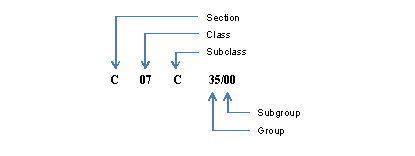
\includegraphics[width=0.60\textwidth,height=30mm]{figs/IPCexample.jpg}
   \caption{An example illustrating the main components of an International Patent Classification code.}   
   \label{fig:ipcexample} 
\end{figure}
%%%%%%%%%%%%%%%%%%%%%%%%%%%%%%%%%%%%%%%%%%%%%%%%%%%%%%%%%%%%%%%%%%%%%%%%%%%%%%%%%

Patents are assigned at least one classification code 
indicating the subject to which the invention relates, this is called Main Code. They may also be assigned further classification and 
indexing terms to give further details of the contents of the invention, which are called Further Codes. 

\paragraph{Citations}
\ \\ 
This section of the patent document contains the list of older patents that are related to the
invention by describing the relevant parts of the prior-art of the invention, or these citations can
be for patents that have been located by the patent examiners and were found to invalidate parts 
of the invention in the initially submitted patent application, where the final version of the patent
get these parts modified or removed.
\section{Generic Information Retrieval}
An information retrieval (IR) system assists users in finding the information they need. Figure~\ref{fig:generalir} illustrates the general IR process. On the collection side, a repository of indexed documents is created from a collection of documents to be searched for. Users formulate the information they need as a query and the IR system answers the query intent. In the matching process, the query and documents representations are compared and the result would be a ranked list of documents. The first attempt at formulation of a query with a particular information need in mind
is often inaccurate and can result in an answer set that does not satisfy the user's information need. 
After reading some of the documents in the initial result set, the query can be reformulated in order to shift the result set toward the information need.
%%%%%%%%%%%%%%%%%%%%%%%%%%%%%%%%%%%%%%%%%%%%%%%%%%
\begin{figure}[htpb]
   \centering
   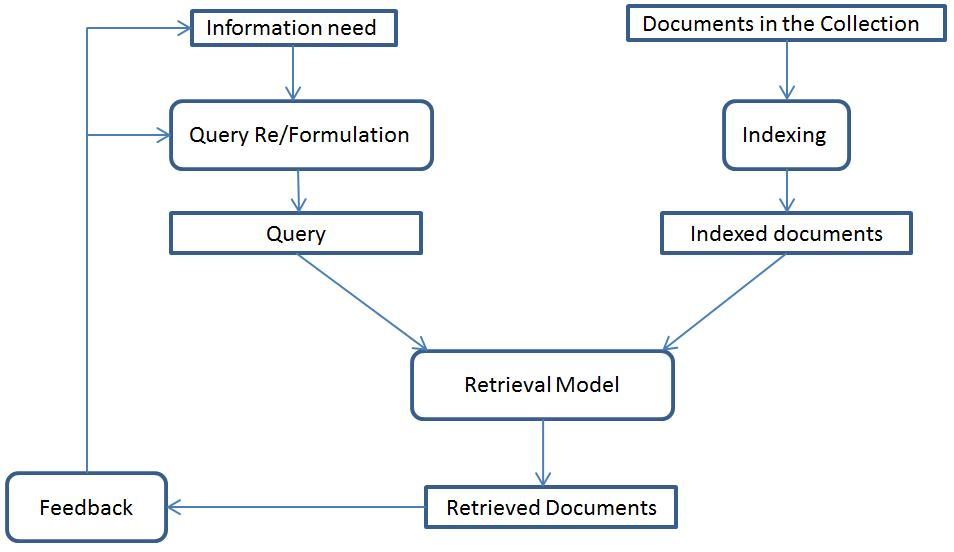
\includegraphics[width=.60\textwidth,height=50mm]{figs/generalIR.jpg}
   \caption{Illustrating of the process in a general IR system.}  
   \label{fig:generalir} 
\end{figure}
\FloatBarrier 
%%%%%%%%%%%%%%%%%%%%%%%%%%%%%%%%%%%%%%%%%%%%%%%%%%
\subsection{Retrieval Models}
\label{subsub:retmodels}
Having constructed an index on a document collection, queries need to 
be matched to documents and a list of answers returned. We need a ranking algorithm based on good mathematical retrieval models to 
return relevant documents at top of the ordered list, leading to high effectiveness. 
Three well-known retrieval models are~\citep[p. 233]{croft2010search}: (1) vector space models (e.g., term frequency and inverse document frequency (TF-IDF)), (2) probabilistic models (e.g., BM25\footnote{BM stands for Best Match, and 25 is just a numbering scheme used by~\cite{robertson1994some} to keep track of weighting variants.}), and (3) Language Models~(LM). 

\paragraph{The Vector Space Model}
\ \\
In a vector space model, documents and queries are represented by vectors of term weights, and the collection is represented by a matrix of term weights as follows: 
\begin{displaymath} 
D_{i}=[d_{i1}, d_{i2}, d_{i3}, \ldots , d_{im}],
\end{displaymath}
\begin{displaymath} 
Q=[q_{1}, q_{2}, q_{3}, \ldots , q_{m}],
\end{displaymath}
\begin{displaymath} 
C=
%\begin{matrix} D_{1} \\ D_{2} \\ D_{3} \\ \vdots\\ D_{N} \\\end{matrix}
\begin{bmatrix}
        d_{11} & d_{12} & d_{13} & \cdots & d_{1m}\\
        d_{21} & d_{22} & d_{23} & \cdots & d_{2m}\\
        d_{31} & d_{32} & d_{33} & \cdots & d_{3m}\\
        \vdots\\
        d_{N1} & d_{N2} & d_{N3} & \cdots & d_{Nm}
     \end{bmatrix},
\end{displaymath}
%\capstartfalse
%\begin{figure}[htpb]
%   \centering
%   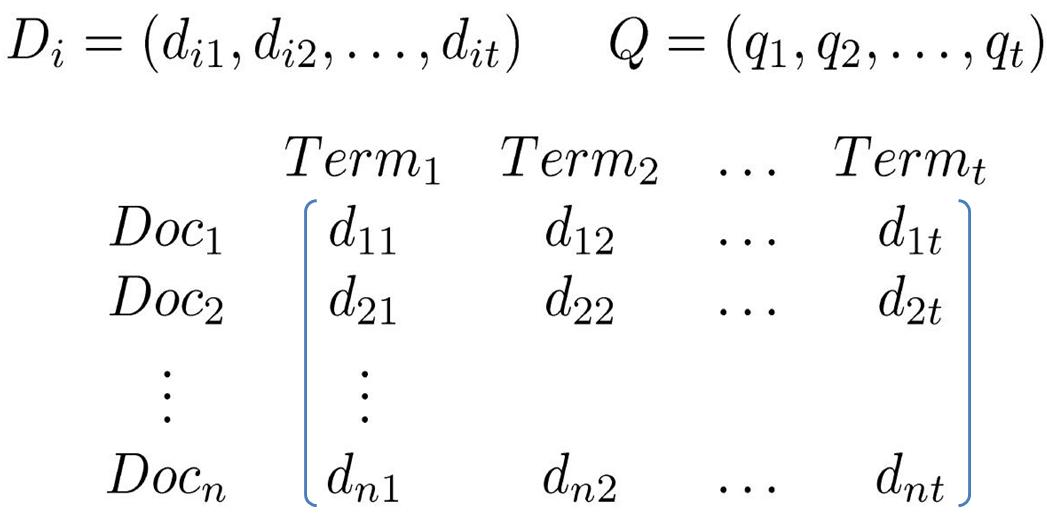
\includegraphics[width=.45\textwidth,height=35mm]{figs/vsm-matrix.jpg}
%\end{figure}
%\capstarttrue
%\FloatBarrier 
\noindent
where $ D_{i} $ is a document in the collection $ C $, $ d_{ik} $ is a weight for each term $ t_{k} $ in the document $ D_{i} $, and $ q_{k} $\footnote{We ignore indices to simplify the further equations in this thesis.} represents a term in the query $ Q $. The collection is represented by the matrix $C_{Nm}$, where $N$ is the number of documents in the collection and $m$ is the number of all vocabularies. If a term does not appear in a document or a query, the weight for that particular term will be zero. 

The TF-IDF weighting function multiplies the occurrence of each term in the document ($ c(t_{k},Di)$)
by the inverse document frequency ($ idf $) measure. $ idf $ measures the importance of a term in the collection: 
\begin{equation}
idf(t_{k})=\log\frac{N+1}{df(t_{k})},
\label{eq:idf}
\end{equation}
where $ df(t_{k}) $ is the number of documents in the collection, which contain at least one occurrence of the term $ t_{k} $, and $ N $ is the number of documents in the collection. 

Given a query $Q$, documents are ranked based on the overlap score measure. The TF-IDF score of a document $D$ is the sum, over all query terms, of the TF-IDF weight of each query term $q$ in $D$. After pivoted normalisation, the TF-IDF score for each document is calculated as follows~\citep{bache2010improving}:
\begin{equation}
TFIDF(Q,D)=\sum\limits_{q \in Q\cap D}\frac{c(q,D)\times idf(q)}{(1-b)+b.\frac{|D|}{avdl}},
\label{eq:tfidf}
\end{equation}
where $ |D| $ is the size of the document (i.e, the number of words) and $ avdl $ is the average document length, $ c(q,D)$ is the number of occurrence of each query term in the document $D$, and $idf(q)$ is the importance of each query term in the collection. TF-IDF model scores a document higher if more query terms are present or these terms are rarer in the collection. The parameter $ b $ is set to 0.75 to be the same as the BM25 model as will be described below.
\paragraph{Probabilistic Models}
\ \\
BM25 is a popular and effective ranking algorithm, which extends the scoring function for the binary independence model~\citep[p. 232]{manning2008introduction} to include document and query term weights. Each document is scored based on the BM25 weighting scheme --- often called the Okapi weighting --- as follows:
\begin{equation}
BM25(Q,D)=\sum\limits_{q \in Q\cap D}\Bigg(\log\frac{N+1}{df(q)}\Bigg)\Bigg(\frac{(k_{1}+1)c(q,D)}{k_{1}((1-b)+b.\frac{|D|}{avdl})+c(q,D)}\Bigg).
\label{eq:idfbm25}
\end{equation}
The variable $ k_{1} $ is a positive tuning parameter that calibrates the document term frequency scaling. The setting of $ k_{1}=0 $ corresponds to a binary model (i.e., no term frequency), and setting a large value for $ k_{1} $ corresponds to using raw term
frequency. The parameter $ b $ is also used for tuning ($ 0 \leq b \leq 1 $) which determines the scaling by document length: $ b = 1 $ corresponds to fully scaling the term weight by the document length, while $ b = 0 $ corresponds to no length normalisation. 

If the query is long, then we might also use similar weighting for query terms. This is appropriate if the queries are paragraph long information needs, but unnecessary for short queries. 
In this case, BM25 weighting function is calculated as follows:
\begin{equation}
BM25(Q,D)=\sum\limits_{q \in Q\cap D}\log\Bigg(\frac{N+1}{df(q)}\Bigg)\Bigg(\frac{(k_{1}+1)c(q,D)}{k_{1}((1-b)+b\frac{|D|}{avdl})+c(q,D)}\Bigg)\Bigg(\frac{(k_{3}+1)c(q,Q)}{k_{3}+c(q,Q)}\Bigg),
\label{eq:idfbm25}
\end{equation}
where $ c(q,Q) $ is the frequency of term $ q $ in the query $ Q $, and $ k_{3} $ being another positive tuning parameter that this time calibrates term frequency scaling of the query. In the equation presented, there is no length normalisation of
queries because retrieval is being done with respect to a single fixed query. The tuning parameters of these equations should ideally be set to optimise performance on a development test collection. That is, we can search for values of these parameters that maximise performance on a separate development test collection (either manually or with optimisation methods such as grid search or something more advanced), and then use these parameters on the actual test collection. In the absence of such optimisation, experiments have shown reasonable values are to set $ k_{1} $ and $ k_{2} $ to a value between 1.2 and 2, and b = 0.75~\citep{manning2008introduction}.
\paragraph{Language Models with Terms Smoothing}
\ \\
The basic idea behind the \textit{Language Modelling} approach is to estimate a language model for each document, and rank documents by the likelihood of the query according to the estimated language model. Here terms are assumed to occur independently, and the probability is the product of the individual query terms given the document model $ M_{D} $ of document $ D $:
\begin{equation}
\label{eq:multinomial}
 P(Q|M_{D}) = \prod\limits_{q\in Q} P(q|M_{D}) 
\end{equation}

\begin{equation}
\label{eq:multinomial}
 P(q|M_{D}) = \frac{c(q,D)}{|D|}
\end{equation}

The overall similarity score for the query and the document could be zero if some of query terms do not occur in the document. However, it is not sensible to rule out a document just because a single query term is missing. For dealing with this, language models make use of smoothing to balance the probability mass between occurrences of terms in documents, and terms not found in the documents.
\\\\
\textit{Jelinek-Mercer smoothing.} Jelinek-Mercer smoothing language model~\citep{zhai2004study} combines the relative frequency of a query term $ q\in Q $ in the document $ D $ with the relative frequency of the term in the collection (\textit{C}) as a whole. With this approach, the maximum likelihood estimate is moved uniformly toward the collection model probability $ P(q|C) $:
\begin{equation}
P(q|M_{D}) = (1-\lambda)\frac{c(q,D)}{|D|}+\lambda P(q|C) 
\label{eq:jmsmoothing}
\end{equation} 
$ c(q,D) $ represents the frequency of term $ q $ in document $ D $. The optimal value of $ \lambda $ depends on both the collection and the query. It is normally suggested as ($ \lambda = 0.1$) for title queries and ($ \lambda = 0.7$) for long queries.
\\\\
\textit{Dirichlet (Bayesian) smoothing (DirS).} As long documents allow us to estimate the language model more accurately, Dirichlet smoothing ~\citep{zhai2004study} smooths them less. If we use the multinomial distribution to represent a language model, the conjugate prior of this distribution is the Dirichlet distribution. This gives:
\begin{equation}
\label{eq:bayessmoothing}
 P(q|M_{D}) = \frac{c(q,D) + \mu P(q|C)}{|D| + \mu}
\end{equation} 

The formula assign negative score to documents that contain the term, but with fewer occurrence than predicted by the collection language model. As $ \mu $ gets smaller, the contribution from the collection model also becomes smaller, and more emphasis is given to the relative term weighting. Precision is more sensitive to $ \mu $ for long queries, especially when $ \mu $ is small. When $ \mu $ is sufficiently large, long queries perform better than short queries. The optimal value of $ \mu $ varies from collection to collection, though in most cases, it is around 2000. The performance is more sensitive to smoothing for verbose queries. Long queries also require more aggressive smoothing to achieve optimal performance. 

\subsection{The Study of Retrievablity}
Retrievability measures indicate how easily a document could be retrieved using a given IR system, while findability measures indicate how easily a document can be found by a user with the IR system~\citep{azzopardi2008retrievability}. Some documents are retrieved by many queries while others may never show up within the top-n ranked results via any query terms that they are relevant for~\citep{lupu2013patent}. When a document is difficult or impossible to retrieve in a particular retrieval model, it is difficult or impossible to retrieve when relevant and this leads to a low recall. 

Essentially, it is desirable that the retrieval system consider all documents with similar retrievability (Gini-Coefficient is used to measure the retrievability) because documents become less retrievable when others become more retrievable. However, two aspects can affect findability: the inherent bias favouring some types of documents over others introduced by the retrieval model, and the failure to correctly capture and interpret the context~\citep{bashir2009improving, bashir2011relationship}. There are certain features that increase access to the corpus by making the retrievability of documents more equal~\citep{bache2010improving}:
\begin{enumerate}
\item Sensitivity to term frequency: A higher frequency of a given query term makes the document more relevant.
\item Length normalization: Incorporation term frequency into a model make it biased to score longer documents higher than shorter documents, so there is a tendency to over-score longer documents. Shorter documents are not penalised when length normalisation is used.
\item Convexity: An IR model will have convexity if it ranks document $ d_{3} $, which has both query words $ w_{1} $ and $ w_{2} $, higher than documents $ d_{1} $ and $ d_{2} $, which just have one of the query words twice. 
\end{enumerate}
Bias of retrieval systems is the characteristic of a system to give preference to certain features of documents, when it ranks results of any given query. For example, \textit{PageRank} favours popular documents by evaluating the number of in-links of web pages in addition to pure content features while \textit{TFIDF} and \textit{OKAPI-BM25} favour large terms frequencies~\citep{bashir2011relationship}.
\paragraph{Retrievablity Measurement}
\ \\
\textit{Retrievability} measures how likely each document $ d $ inside a collection $ D $ can be retrieved within the top c ranked results for all queries in $ Q $. $ r(d) $ defines as follows:
\[
r(d)=\sum_{q \in Q}f(k_{dq},c)
\]
where $ k_{dq} $ is the rank of $ d $ in the result set of query $ q \in Q $, $ c $ denotes the maximum rank that a user is willing to proceed down the ranked list. The function $ f(k_{dq},c) $ returns a value of 1 if $ k_{dq} \leq c $, and 0 otherwise. \textit{Retrievability} inequality can be analysed using the \textit{Lorenz} Curve. Documents are sorted according to their retrievability score in ascending order, plotting a cumulative score distribution. If the retrievability of documents is distributed equally, then the Lorenz Curve will be linear. The more skewed the curve, the greater the amount of inequality or bias within the retrieval system. The Gini coefficient $ G $ is used to summarize the amount of bias in the Lorenz Curve, and is computed as follows:
\begin{equation}
G=\frac{\sum_{i=1}^n(2.i-n-1).r(d_{i})}{(n-1)\sum_{j=1}^nr(d_{j})}
\end{equation}
\noindent
where $ n=|D| $ is the number of documents in the collection sorted by $ r(d) $. If $ G=0 $, then no bias is present because all documents are equally retrievable. If $ G=1 $, then only one document is retrievable and all other documents have $ r(d)=0 $. By comparing the Gini-Coefficients, we can analyse the retrieval bias imposed by the underlying retrieval functions on a given document collection.

\label{subsub:retrievability}

\subsection{Query Expansion}
One solution to the significant term mismatch between the query and the relevant documents is query expansion (QE)~\citep{Efthimiadis1996}, which has been effective in many retrieval tasks. The idea of QE is to add more terms to the original user's query to increase the probability of matching of the query terms with relevant documents, with the objective of improving retrieval effectiveness. The expansion terms can be selected from a feedback process or from external sources such as Wikipedia, or dictionaries~\citep{cao2008selecting}. Original queries should be expanded by good terms, unless it can lead to retrieval of irrelevant documents.
\paragraph{Feedback-based Query Expansion}
\ \\
An initial query can be expanded using a feedback from users --- relevance feedback --- or automatically from top $ k $ ranked retrieved documents, assuming they are relevant to the query --- pseudo relevance feedback (PRF)~\citep{manning2008introduction}. Getting feedback from  users needs user studies and interaction while pseudo relevance feedback is an automated process without user interaction.
\begin{figure}[t!]
%[htpb]
   \centering
   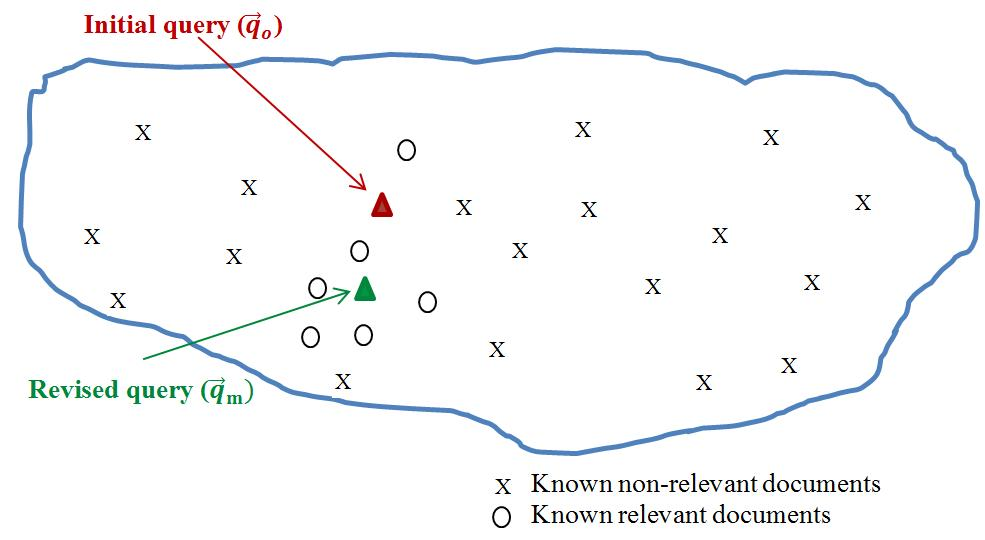
\includegraphics[width=0.65\textwidth,height=50mm]{figs/rocchio.jpg}
   \caption{Rocchio algorithm for relevance feedback. Some documents have been labelled as relevant and irrelevant and the initial query vector is moved in response to this feedback~\citep{manning2008introduction}.}  
   \label{fig:rocchio} 
\end{figure}
\FloatBarrier 
%\noindent
\textit{The Rocchio Algorithm for Relevance Feedback}: The Rocchio
algorithm \citep{Salton1971} is a classic algorithm of relevance feedback
used mainly for query expansion. In brief, it provides a method of
incorporating relevance feedback information into the vector space
model representing a query~\citep{manning2008introduction}. 
The Rocchio algorithm is used to modify the query by the partial knowledge of known relevant and irrelevant~\footnote{In this thesis, we use irrelevant and non-relevant interchangeably for documents that are not relevant to the query.} documents; the goal is to move the query closer to the centroid of the relevant documents but further from irrelevant documents (Figure \ref{fig:rocchio}). The modified query $ \vec{q}_m $ is:
%\[ 
\begin{equation}
\label{eq:rocchio}
 \vec{q}_{m} = \alpha  \vec{q}_{0} + \beta\frac{1}{|D_{r}|}\sum\limits_{\vec{d_{j}}\in D_{r}} \vec{d_{j}} - \gamma\frac{1}{|D_{irr}|}\sum\limits_{\vec{d_{j}}\in D_{irr}} \vec{d_{j}},
  \end{equation}
 %\tag{2.1}\label{eq:rocchio}
 %\]  
where $ q_{0} $ is the original query vector; $ D_{r} $ and $ D_{irr} $ are the set of known relevant and irrelevant documents, respectively; and $ \alpha $, $ \beta $, and $ \gamma $ are weights attached to each term. These control the balance between trusting the judged document set versus the query: if we have a lot of judged documents, we
would like higher $ \beta $ and $ \gamma $~\citep{manning2008introduction}. 

PRF is typically used in Rocchio algorithm. However, it is important to distinguish between good expansion terms and bad ones. Distinguishing between expansion terms only based on their distribution in the feedback documents (i.e., extracting the most frequent terms) and in the whole collection (i.e., extracting the most specific terms) is not sufficient. It can be considered as a term classification problem to separate good expansion terms from others directly according to their potential impact on the retrieval effectiveness; hence, we can apply supervised learning methods for term selection. Classifiers like support vector machines (SVM)~\citep{cao2008selecting}, Na\"ive Bayes and Logistic Regression~\citep{he2009finding} can be used to classify terms and feedback documents.  
\paragraph{Query Expansion by External Resources}
\ \\
The most common form of query expansion is a global analysis, using dictionaries, WordNet, Wikipedia, or other thesaurus. For each term $ t $ in a query, the query can be automatically expanded with synonyms and related words of $ t $ from the thesaurus. Use of a thesaurus can be combined with ideas of term weighting; for instance, one might weight added terms less than original query terms~\citep{manning2008introduction}.

\subsection{Query Reduction}
In general, retrieval effectiveness for long queries is often lower than retrieval effectiveness for shorter keyword queries because the additional information provided in verbose queries is more likely to confuse current search engines rather than help them. Query reduction (QR), a technique for dropping unnecessary query terms from long queries, improves the performance. 

A common approach to reduce verbose queries is selecting a subset of a long query (or sub-query). A search engine performs more precisely when just the key concepts are used as a query rather than a long query. Hence, the identification of the key query concepts has a positive impact on the retrieval performance for verbose queries. Extracting the key query concepts can be done by learning to identify key concepts in long queries using a variety of features~\citep{bendersky2008discovering}. We can choose effective subsets in a query by analysing all the subsets of terms from the original query (sub-queries), and identifying the most promising sub-query to replace the original long query. For ranking sub-queries, an algorithm based on the SVM classification is used~\citep{kumaran2009reducing}. In this approach, the quality of query reduction depends on the performance of the predictor and ranking algorithm~\citep{balasubramanian2010exploring}. 

As the other approach, we can use query term ranking techniques to select effective terms from a verbose query by ranking them. A vast number of rankings are possible given different settings of individual term weights; for example, we can train a regression model to weight all query words of a verbose query~\citep{lease2009regression}. We can also assign weights to concepts by learning the importance of concepts underlying
the verbose query~\citep{bendersky2010learning}.

%\subsubsection{Query Reformulation}
%\input{query_reform}

\subsection{IR Evaluation Metrics}
A retrieval system is evaluated considering a set of relevance judgements, a binary assessment of either \textit{relevant} or \textit{irrelevant} for each query-document pair. An ideal retrieval system can retrieve all relevant documents. Table \ref{tab:contengency} is the contingency table, where:\\\\
\textit{True Positive (tp)}: documents which are relevant and the system retrieves them.\\
\textit{False Negative (fn)}: documents which are relevant but the system does not retrieve them. \\
\textit{False Positive (fp)}: documents which are non-relevant but the system retrieves them.\\
\textit{True Negative (tn)}: documents which are non-relevant and the system does not retrieve them. 
\begin{table*}[htpb]
  \centering
  \input table/contingency.tex
  \caption{Contingency table.}
  \label{tab:contengency}
\end{table*}
\FloatBarrier 
\paragraph{Precision and Recall}
\ \\
Precision and recall are the most frequent and basic measures for information retrieval effectiveness. They are calculated with respect to what IR system returns as a set of documents for a query.\\
\textit{Precision (P)} is the fraction of retrieved documents that are relevant:
\[
Precision (P)=\frac{\sharp(relevant \: items \: retrieved)}{\sharp(retrieved \: items)}=\frac{tp}{tp+fp}=P(relevant|retrieved)
\]
\textit{Recall (R)} is the fraction of relevant documents that are retrieved:
\[
Recall (R)=\frac{\sharp(relevant \: items \: retrieved)}{\sharp(relevant \: items)}=\frac{tp}{tp+fn}=P(retrieved|relevant)
\]
For many prominent applications, particularly web search, good results on the first page or the first three pages are important than all relevant documents. So, they wish to look at precisions and recalls over a series of different rank cut-offs rather than to look at the entire retrieved set. This is referred to as ``Precision/Recall at k'', for example ``Precision/Recall at 10''. 
\begin{equation}
precision@k=\frac{\sharp(documents \: retrieved \: and \: relevant \: up \: to \: rank \: k)}{k}
\end{equation}
\begin{equation}
recall@k=\frac{\sharp(documents \: retrieved \: and \: relevant \: up \: to \: rank \: k)}{\sharp(documents \: relevant)}
\end{equation}
\paragraph{Average Precision and Mean Average Precision (MAP) }
\ \\
We can measure MAP by calculating Average Precision on retrieval results. Average Precision is the average of precision at each point where a relevant document is found is computed as:
\begin{equation}
Avg. \: precision=\frac{\sum_{r=1}^{N}(P(r)\times rel(r))}{n}
\end{equation}
\noindent
where $ r $ is the rank, $ N $ the number of documents retrieved, $ rel(r) $ a binary function of the document relevance at a given rank, $ P(r) $ is precision at a given cut-off rank $ r $, and $ n $ is the total number of relevant documents.

Then, for a given set of queries, $ Q $, $ MAP $ can be calculated by:
\begin{equation}
MAP(Q)=\frac{\sum_{q\in Q}Avg. \: precision(q)}{|Q|}
\end{equation}
\noindent
where $ q $ is a query in a set of queries $ Q $.

%------------------- Patent-specific IR ---------------------

\section{Patent-specific Information Retrieval}
\label{subsec:patentir}
Patent retrieval differs from a generic retrieval due to specific characteristics of patents. For instance, in patent prior art search the query is as long as a patent document, which makes the query (re)formulation more difficult compared to a web search. Patents have some specific features that can be yielded in retrieval, which we will  discuss in this section.

\subsection{The Study of Retrievablity for Patents}
Rerievability is specifically critical in recall oriented applications like patent retrieval or legal settings. In these cases, the focus of a system is to retrieve all documents that are relevant rather than to retrieve a subset of documents that the best satisfy the query intent.
Hence, all documents should at least potentially be retrievable via correct query terms. Designing retrieval systems for recall oriented tasks has been emphasised in recent years~\citep{fujii2007introduction, kontostathis2008effect}. Before designing a new or using an existing retrieval system for recall oriented applications, one needs to analyse the effects of the retrieval system bias as well as the overall retrievability of all documents in the collection using the retrieval function at hand.

In retrievability, we analyse documents specifically with respect to relevant and irrelevant queries to identify whether highly retrievable documents are really highly retrievable, or whether they are simply more accessible from many irrelevant queries rather than from relevant queries. Experiments show that about 90\% of patent documents which are highly retrievable across all types of queries, are not highly retrievable on their relevant query sets~\citep{bashir2009analyzing}.

Experiments with different collections of patent documents suggest that query expansion with pseudo relevance feedback can be used as an effective approach for increasing the findability of individual documents and decreasing the retrieval bias. Pseudo relevance feedback documents are identified using cluster-based~\citep{bashir2009improving} or terms-proximity-based methods~\citep{bashir2010improving}.

Another study~\citep{bache2010improving} analyses the relationship between retrievability and effectiveness-based measures (Precision, MAP). Results show that the two goals of maximising access and maximising performance are quite compatible. They further conclude that a reasonably good retrieval performance can be obtained by selecting parameters that maximise retrievability (i.e., when there is the least inequality between documents according to Gini coefficient given the retrievability values). Their results support the hypothesis that retrieval functions can be effectively tuned using a retrievability-based measure without recourse to relevance judgments, making it an attractive alternative for automatic evaluation.


\subsection{Initial Query Formulation}
%Query or topic is the the request for information in any retrieval system. An effective query can lead in retrieving the required information. Queries formulated by users are not usually optimal for retrieval process, therefore, they need to be transformed by techniques such as query expansion or query reduction. 
The patent prior art search begins with a full patent application as a query. A full text as a query is a challenge compared to a classical IR, since it is not focused on the information that the user needs. In order to achieve good retrieval results, it is important to extract the best representative text with the proper weights. Therefore, query generation based on query document is essential to reduce the difficulty of formulating effective queries by users. 
%The query created before the retrieval can be modified or enhanced after retrieval. In this section, the initial query formulation will be discussed and in the next section, post-retrieval query reformulation will be covered. 
\\\\
\textbf{Which fields in patent application are more effective to extract query terms}
\ \\
A special characteristic of patent documents is their structural information. They mainly have different fields such as title, abstract, description, and claims. Different fields use different type of language for describing the invention. Abstract and description use more technical terminology while claim field usually uses a legal jargon. Structured indexing keeps the field structure in the index, which allows searching specific fields instead of searching in full document. Separate fields for meta-data (Section \ref{sec:metadata} ) like IPC code and author can help to retrieval effectiveness~\citep{magdy2010exploring}. 

Early patent search tasks mainly considered claims to build the query, the same as what examiners start the novelty process~\citep{konishi2005query, takaki2004associative, mase2005proposal, fujii2007enhancing}, whereas recent works have showed that building queries from description field is more useful in patent retrieval (considering background summary in US patents equivalent to description field in European patents.)~\citep{xue2009transforming, xue2009automatic, mahdabi2011building}. Another research showed that extracting terms according to $ log(tf)idf $ scores from every field of the query patent, and giving higher importance to terms extracted from the abstract, claims, and description fields than to terms extracted from the title field, is an effective way of constructing a search query~\citep{cetintas2012effective}. The other experiment showed that discarding description from query improves MAP up to 30\% because the description contains more noise than information~\citep{gobeill2010simple}. They also showed that claims are more informative and title is poorly informative in retrieval.   


\paragraph{Using Phrases instead of Terms}
\ \\
Most of query formulation techniques rely on terms, but encouraging results have been obtained using phrases recently~\citep{becks2010phrases}. Early results demonstrated that an NLP-based grouping of terms can increase the performance compared to the bag-of-words approach, though the increase is smaller than in a non-patent collection~\citep{osborn1997evaluating}. Another task could improve retrieval effectiveness by adding syntactic phrases in the form of dependency triples, to a bag-of-words representation~\citep{d2011combining}. Key Phrase Extraction (KPE) algorithms is another way to form a query based on phrases. A list of phrases, generated by a KPE algorithm, can succinctly represent a complex and lengthy patent. ~\citep{verma2011applying}.

\paragraph{Diverse Query Generation}
\ \\
In this approach, the focus is on generating diverse queries that can improve overall retrieval effectiveness in sessions rather than generating a single best query that can retrieve more relevant documents from a single retrieval result (i.e., more relevant documents in aggregated retrieval results obtained by multiple queries in a session). Diverse query generation is important because query documents typically contain several different aspects (or topics) and different types of relevant documents may be related to these aspects. To identify aspects, 500 top terms based on their tf-idf rank, are clustered into $ n $ sets with respect to their similarity. Each distinct sets of terms represents one query aspect, then top $ k $ retrieved documents for each sub-query consider as pseudo-relevant documents (PRD) and those ranked below the top $ k $ are non-relevant documents (NRD). Then the query is generated by decision tree. ~\citep{kim2014searching, kim2014diversifying}.

\subsection{Query Expansion for Patents}
Although a query is very long in patent prior art search, a significant term mismatch between queries and relevant documents has reported in~\citep{roda2010clef, magdy2010exploring}. The QE is a suggested solution to cope with the term mismatch problem; however, most of the QE techniques were ineffective to improve the performance in patent domain~\citep{kishida2003experiment, konishi2005query}. We review previous works on the QE techniques for the patent search here.
\paragraph{Query Expansion by Pseudo Relevance Feedback}
\ \\
Previous studies~\citep{magdy2011study} have discussed that PRF is ineffective for patent prior art search. Since the retrieval effectiveness is low at initial retrieval, the assumption that top $ k $ documents are relevant is invalid and leads in adding noise to the query; hence, the improvement using PRF is insignificant. The solutions proposed to cope with this problem are as follows:
\begin{list}{-}{}
\item \textbf{Selecting documents for PRF based on cluster analysis:} In this approach, a document that can cluster lots of high similar documents is considered relevant and a document that has no nearest neighbour or some neighbours with low similarity is considered irrelevant~\citep{lee2008cluster}. In patent domain, where there is a large vocabulary diversity for expressing an invention, the idea can be improved by intra-cluster similarity rather than only on the basis of their size~\citep{bashir2009improving}. 
\item \textbf{Selecting patents for PRF based on their similarity with query patent via specific terms:} In this approach, patents for PRF are identified based on their similarity with query patents over a subset of terms, rather than the overall document similarity. The success of this approach highly depends on selecting appropriate terms from patent query, which produce the best PRF candidates that can help in improving retrievability during QE~\citep{bashir2010improving}. Experiments show a significant improvement for Gini coefficient, which is used to measure retrievability, but there is no report on other main measures (e.g., MAP and recall).
\item \textbf{Identyfying expansion terms: } 
\ \\
Term proximity information can be used to identify expansion terms. Given a patent query, first, an initial query is generated by taking, for example, claim terms; then a query-specific lexicon based on definitions of the IPC is created.
Among many terms in the lexicon, only expansion terms identified by two adjacency operators used in patent examination\footnote{Patent examiners use term proximity heuristics in their
searches in Boolean retrieval model in order to reward a
document where the matched query terms occur close to
each other. Two forms of adjacency operators are used in
Boolean retrieval model to address proximity. `ADJn' operator which searches for terms within \textit{n} words proximity in
the order specified, and `NEARn' operator, which searches
for the terms within \textit{n} words, in either order.} (i.e., `ADJn' and `NEARn') are used for query expansion~\citep{mahdabi2013leveraging}.
\item \textbf{Predicting the effectiveness of feedback documents: } 
\ \\
In patent retrieval, the MAP is very low at initial retrieval; hence the top retrieved documents are not essentially relevant. 
As a result, there is a high
chance that we use irrelevant documents for expansion in PRF. Recently,
machine learning methods like regression are used to improve the PRF by predicting the effectiveness of a feedback document~\citep{mahdabi2012learning}.
\end{list}
Random indexing to identify terms to use for query expansion~\citep{sahlgren2002english} and expansion using noun phrases~\citep{mahdabi2012automatic} are the other techniques to improve the effectiveness of standard query expansion for prior art search. 
\paragraph{Query Expansion by External Resources}
\ \\
Some external resources like WordNet~\citep{miller1990introduction}, which were reported to improve retrieval effectiveness in several IR research investigations, show insignificant change to overall retrieval effectiveness, but a degree of improvement for some topics in patent domain. \cite{magdy2011study} applied the idea of automatically generating the synonyms set (SynSet) using parallel manual translations to create possible synonyms sets (in CLEF-IP collection, some sections in some patents are translated into three languages: English, French, and German). Although this idea presents better results compared to WordNet, there is still a little improvement in retrieval effectiveness. The only QE task, which achieves the best results, uses a combination of PRF and QE with translation of terms and phrases from German and French~\citep{jochim2011expanding}.


\subsection{Query Reduction for Patents}
Query reduction is a solution for problems with using a full verbose patent as a query: it is not focused on information needed by the user, and a verbose query may cover more than one topic.

\begin{list}{-}{}

\item \textbf{Query Segmentation :} Decomposing each patent query into coherent sub-topics segments-using TextTiling~\citep{hearst1997texttiling}-is a solution to make long ambiguous queries focused on the information need. Sub-topic segments can be used as separate queries (query stream) for initial retrieval, then the retrieval results from each of the individual streams are merged to construct the final ranked list for the whole original query. Using each sub-topic as a query stream enables a retrieval model to retrieve related documents from the collection in a more precise way and also allow the PRF algorithm to work on a more focused set of pseudo-relevant documents~\citep{takaki2004associative, ganguly2011united}. Another work adapted pseudo relevance feedback for query reduction by decomposing a patent application into constituent text segments and computing the Language Modelling (LM) similarities by calculating the probability of generating each segment from the top ranked documents. The least similar segments from the query removed from the query, hypothesizing that removal of segments most dissimilar to the pseudo-relevant documents can increase the precision of retrieval by removing non-useful context, while still retaining the useful context to achieve high recall as well~\citep{ganguly2011patent}.

\item \textbf{Patent Summarization :} This approach assumes that the patent summary (using TextTiling) reflects the main topic as well as the subtopics of a patent document in a concise manner. Then, language model for the query, collection, and each summary are generated~\citep{mahdabi2011report}. 

\end{list}



%\subsubsection{Query Reformulation for Patents}
%\input{query-reform-p}

\subsection{The Use of Metadata}
The main textual content of patent documents is known to be difficult to process with traditional text processing and text retrieval techniques, but patents contain additional material, such as: tables, mathematical and chemical formulas, citations, technical drawing, meta-data, e.g., applicant, inventor, Intentional Patent Classification (IPC) codes, and publication date, that can be used to improve the retrieval. In this section, the use of patent meta-data to improve the retrieval has been explained.
\paragraph{The Use of Citation}
\ \\
The most successful use of metadata to date is the citation lists in order to learn patterns of relevance ~\citep{lupu2013patent}. The patent collection is a very dense network of citations creating a set of interrelations particularly interesting to exploit during a prior art search. The large majority of patents are continuations of previous works and patents. The citation relations make this development process
visible. Similarly, fundamental patents which open new technologies sub-fields are exceptional but tends to be cited very frequently in the whole sub-field during years. Citation graph of a patent collection is used for identifying patent thickets, i.e. the patent portfolios of several companies overlapping on a similar technical aspect. Related patents can be inferred from the overall citation network of a patent collection. If a new patent applicant belonging to this patent ticket appears, it is very likely that the most relevant prior art documents are already
present in this patent thicket~\citep{lopez2009multiple}.

The patents cited in the description of the topic patent are used as relevant documents, because citations are usually prior arts for a citing patent. Only citations which are in the collection can be helpful in the retrieval process. The idea of \textit{PageRank}-identifying authoritative pages by analysing hyperlink structure on World Wide Web\_ can be used for citations. A patent, which is cited by a large number of other patents, is more important. Text-based and citation-based scores combined to compute the ranking score for documents~\citep{fujii2007enhancing, fujii2007integrating}.

Citation texts for patents are a whole paragraph. Therefore, for each patent document presented and cited in the collection, the entire paragraph of citation can be appended to the textual material of the cited patent. A boolean feature uses to indicate weather a cited patent in query patent has retrieved, then this document can get a higher weight at any future post-ranking process. Due to the limited number of citation texts, this approach showed just a trivial improvement~\citep{lopez2009multiple}. However, citation information does not always presented in the patent application and this method can not be used in real life patent search and initial citations by the applicants may not consider relevant by patent examiners~\citep{magdy2010applying, magdy2011simple}. 

Similar tasks also indicated improvement in 'MAP' and 'Recal' using citations in patent retrieval~\citep{gobeill2010simple, gurulingappa2010prior}. 
\paragraph{The Use of IPC Codes}
\ \\
Patents are classified by the patent offices into large hierarchical classification schemes based on their area of technology. The use of patent
classification has two major benefits. The first is that the classifications provide access to concepts rather than words, such that even
if the same word or phrase is commonly used in two technology areas, patent classifications will provide the context of its use. In effect, they
allow the search space of patents to be reduced, by allowing the user to exclude from the search process patents in classes not related to
the search topic at hand~\citep{lopez2010patatras}. The second major benefit is the language independence provided by classifications, as classification symbols can be mapped to multiple languages~\citep{DBLP:conf/clef/DhondtV10}. This allows patent searchers to conduct reasonably effective retrieval even in languages that they do not understand. All previous works, considered IPC code in their search, reported improvement in retrieval effectiveness~\citep{harris2010comparison, harris2011using, harris2009role, fujita2005revisiting, graf2010knowledge, herbert2010prior, kang2007cluster, verma2011applying}. It has also reported that using complete IPC code leads in better results than just 4-digit code~\citep{ gobeill2010simple}.
\paragraph{The Use of Images}
\ \\
For the purposes of the search for innovation, we are interested in all forms of information. Some technology areas rely information present in images (flowcharts and diagrams), so, beyond text data, image processing tasks also can contribute to the search. Graph-based measure has a higher discriminative power, but higher computational costs than the text-based measures~\citep{lupu2013evaluating}.

\label{sec:metadata}

\subsection{Multilinguality}
The interest in multilingual patent search arises from their international and multilingual nature (the European patent office-EPO-makes patent text available in three languages: English, French, and German). Patents on the same topic may be published in different countries in different languages, and it is important for patent examiners to be able to locate relevant existing patents whatever language they are published in. Therefore an important topic in patent retrieval is Cross-Language Information Retrieval (CLIR), where the topic is a patent application in one language and the objective is to find relevant prior-art patents in another language ~\citep{lupu2013patent,joho2010survey, roda2010clef, DBLP:conf/clef/PiroiLHSMF12}. In recent years machine
translation (MT) has become established as the dominant technique for translation in CLIR, which usually achieve better CLIR effectiveness than dictionary-based translation (DBT) methods. However, translation using MT is time consuming and resource intensive for cross language patent retrieval (CLPR), where the query text can often take the form of a full patent application running to tens of pages. Applying IR text pre-processing like stop word removal and stemming to the MT training corpus prior to the training phase can lead to a significant decrease in the MT computational~\citep{magdy2013studying}.




\subsection{Multi-stage Retrieval}
It is common to use patent meta-data and non-textual features as pre and post processing steps of text-based retrieval techniques~\citep{lopez2009multiple}. Many patent retrieval tasks re-rank the top retrieved documents from initial retrieval stage based on additional patent feature~\citep{lopez2010experiments}, claim structure ~\citep{mase2005proposal}, and considering IPC information of patent and its neighbours to retrieve similar patents~\citep{verma2011exploring}. 

\subsection{Evaluation Metrics for Patent Retrieval}
The simplest solution to measure the performance in a recall focused IR task is to evaluate the recall, however, it fails to reflect how early a system retrieves the relevant documents and without precision, returning a perfect recall is invalid~\citep{Suominen08t.:critical}. Although recall is the objective for such applications, the score should be able to distinguish between systems that retrieve relevant documents earlier than those that retrieve them later. For recall-oriented IR applications, the problem is viewed as a ranking problem with a cut-off for a maximum number of documents to be checked $ N_{\max} $.\\\\
\textbf{Patent Retrieval Evaluation Score}
\ \\
\begin{figure}[t!]
   \centering
%   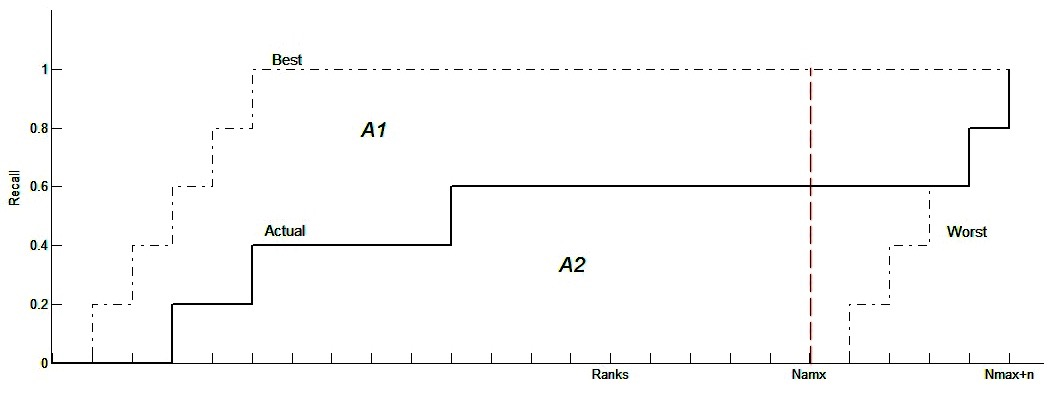
\includegraphics[width=1\textwidth,height=50mm]{figs/pres.jpg}
   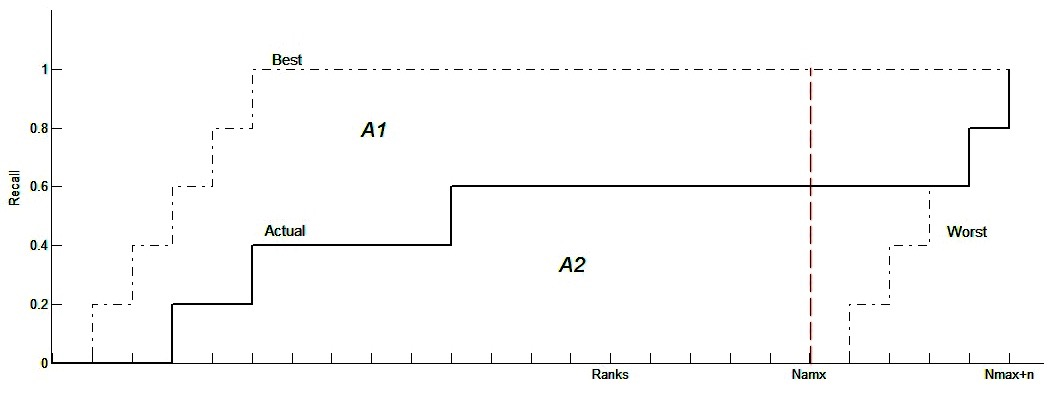
\includegraphics[scale=.37]{figs/pres.jpg}
   \caption{PRES curve is bounded between the best case and the new defined worst case~\citep{magdy2010pres}.}  
   \label{fig:pres} 
\end{figure}
%\FloatBarrier 
Patent retrieval evaluation score (PRES)~\citep{magdy2010pres} is a novel metric for evaluating recall-oriented IR applications, which derived from the normalised recall measure ($ R_{norm} $). It measures the ability of a system to retrieve all known relevant documents earlier in the ranked list. Unlike MAP and recall, PRES is dependent on the relative effort exerted by users to find relevant documents. This is mapped by $ N_{\max} $ (Equation \ref{eq:pres}), which is an adjustable parameter that can be set by users and indicates the maximum number of documents they are willing to check in the ranked list. PRES measures the effectiveness of ranking documents relative to the best and worst ranking cases, where the best ranking case is retrieving all relevant documents at the top of the list, and the worst is to retrieve all the relevant documents just after the maximum number of documents to
be checked by the user ($ N_{\max} $). The idea behind this assumption is that getting any relevant document after $ N_{\max} $ leads to it being missed by the user, and getting all relevant documents after max leads to a zero recall, which is the theoretical worst case scenario. 
%Figure 1 shows an illustrative graph of how to calculate PRES, where 
PRES is the area between the actual and worst cases ($ A_{2} $) divided by the area between the best and worst cases ($ A_{1}+A_{2} $).
$ N_{\max} $ introduces a new definition to the quality of ranking of relevant results, as the ranks of results are relative to the value of $ N_{\max} $. Any relevant document not retrieved in the top N max is assumed to be the worst case (Figure~\ref{fig:pres}).
For example, getting a relevant document at the rank 10 will be very good when $ N_{\max}=1000 $, good when $ N_{\max}=100 $, but bad when $ N_{\max}=15 $, and very bad when $ N_{\max}=10 $. Systems with a higher recall can achieve a lower PRES value when compared to systems with a lower recall but a better average ranking. The PRES value varies from $ R $ to $ \frac{nR^{2}}{N_{\max}} $, where $ R $ is the recall, according to the average quality of ranking of relevant documents.
\begin{equation}
\label{eq:pres}
PRES=\frac{A_{2}}{A_{1}+A_{2}}=1-\frac{\frac{\sum r_{i}}{n}-\frac{n+1}{2}}{N_{\max}},
\end{equation}
where $ r_{i} $ is the rank at which the $ i $th relevant document is retrieved, $ N_{\max} $ is the maximum number of retrieved documents to be checked by the user (i.e. the cut-off number of retrieved documents) and $ n $ is the total number of relevant documents.


%\input{background1}

%\subsection{Retrieval Models}
%\label{subsub:retmodels}
%%Having constructed an index on a document collection, queries need to 
be matched to documents and a list of answers returned. We need a ranking algorithm based on good mathematical retrieval models to 
return relevant documents at top of the ordered list, leading to high effectiveness. 
Three well-known retrieval models are~\citep[p. 233]{croft2010search}: (1) vector space models (e.g., term frequency and inverse document frequency (TF-IDF)), (2) probabilistic models (e.g., BM25\footnote{BM stands for Best Match, and 25 is just a numbering scheme used by~\cite{robertson1994some} to keep track of weighting variants.}), and (3) Language Models~(LM). 

\paragraph{The Vector Space Model}
\ \\
In a vector space model, documents and queries are represented by vectors of term weights, and the collection is represented by a matrix of term weights as follows: 
\begin{displaymath} 
D_{i}=[d_{i1}, d_{i2}, d_{i3}, \ldots , d_{im}],
\end{displaymath}
\begin{displaymath} 
Q=[q_{1}, q_{2}, q_{3}, \ldots , q_{m}],
\end{displaymath}
\begin{displaymath} 
C=
%\begin{matrix} D_{1} \\ D_{2} \\ D_{3} \\ \vdots\\ D_{N} \\\end{matrix}
\begin{bmatrix}
        d_{11} & d_{12} & d_{13} & \cdots & d_{1m}\\
        d_{21} & d_{22} & d_{23} & \cdots & d_{2m}\\
        d_{31} & d_{32} & d_{33} & \cdots & d_{3m}\\
        \vdots\\
        d_{N1} & d_{N2} & d_{N3} & \cdots & d_{Nm}
     \end{bmatrix},
\end{displaymath}
%\capstartfalse
%\begin{figure}[htpb]
%   \centering
%   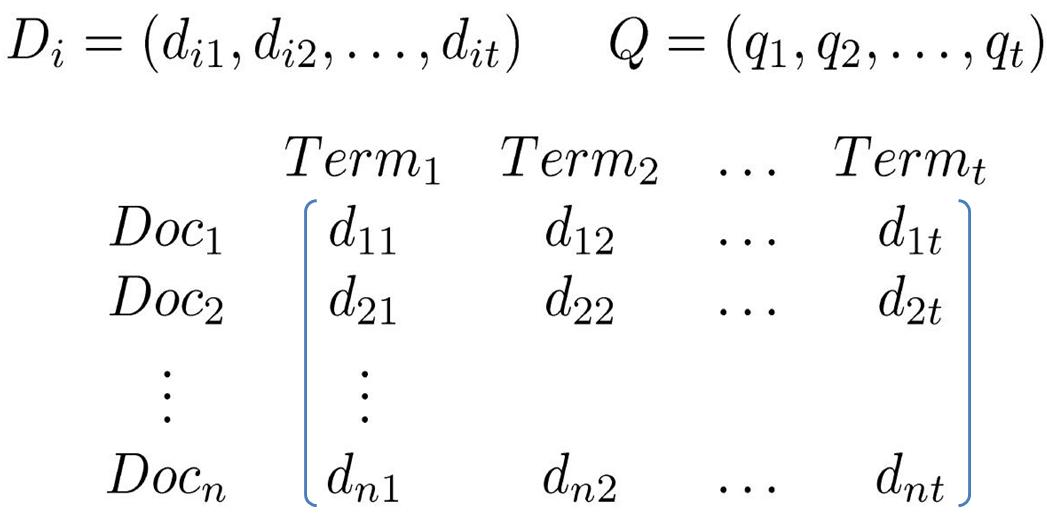
\includegraphics[width=.45\textwidth,height=35mm]{figs/vsm-matrix.jpg}
%\end{figure}
%\capstarttrue
%\FloatBarrier 
\noindent
where $ D_{i} $ is a document in the collection $ C $, $ d_{ik} $ is a weight for each term $ t_{k} $ in the document $ D_{i} $, and $ q_{k} $\footnote{We ignore indices to simplify the further equations in this thesis.} represents a term in the query $ Q $. The collection is represented by the matrix $C_{Nm}$, where $N$ is the number of documents in the collection and $m$ is the number of all vocabularies. If a term does not appear in a document or a query, the weight for that particular term will be zero. 

The TF-IDF weighting function multiplies the occurrence of each term in the document ($ c(t_{k},Di)$)
by the inverse document frequency ($ idf $) measure. $ idf $ measures the importance of a term in the collection: 
\begin{equation}
idf(t_{k})=\log\frac{N+1}{df(t_{k})},
\label{eq:idf}
\end{equation}
where $ df(t_{k}) $ is the number of documents in the collection, which contain at least one occurrence of the term $ t_{k} $, and $ N $ is the number of documents in the collection. 

Given a query $Q$, documents are ranked based on the overlap score measure. The TF-IDF score of a document $D$ is the sum, over all query terms, of the TF-IDF weight of each query term $q$ in $D$. After pivoted normalisation, the TF-IDF score for each document is calculated as follows~\citep{bache2010improving}:
\begin{equation}
TFIDF(Q,D)=\sum\limits_{q \in Q\cap D}\frac{c(q,D)\times idf(q)}{(1-b)+b.\frac{|D|}{avdl}},
\label{eq:tfidf}
\end{equation}
where $ |D| $ is the size of the document (i.e, the number of words) and $ avdl $ is the average document length, $ c(q,D)$ is the number of occurrence of each query term in the document $D$, and $idf(q)$ is the importance of each query term in the collection. TF-IDF model scores a document higher if more query terms are present or these terms are rarer in the collection. The parameter $ b $ is set to 0.75 to be the same as the BM25 model as will be described below.
\paragraph{Probabilistic Models}
\ \\
BM25 is a popular and effective ranking algorithm, which extends the scoring function for the binary independence model~\citep[p. 232]{manning2008introduction} to include document and query term weights. Each document is scored based on the BM25 weighting scheme --- often called the Okapi weighting --- as follows:
\begin{equation}
BM25(Q,D)=\sum\limits_{q \in Q\cap D}\Bigg(\log\frac{N+1}{df(q)}\Bigg)\Bigg(\frac{(k_{1}+1)c(q,D)}{k_{1}((1-b)+b.\frac{|D|}{avdl})+c(q,D)}\Bigg).
\label{eq:idfbm25}
\end{equation}
The variable $ k_{1} $ is a positive tuning parameter that calibrates the document term frequency scaling. The setting of $ k_{1}=0 $ corresponds to a binary model (i.e., no term frequency), and setting a large value for $ k_{1} $ corresponds to using raw term
frequency. The parameter $ b $ is also used for tuning ($ 0 \leq b \leq 1 $) which determines the scaling by document length: $ b = 1 $ corresponds to fully scaling the term weight by the document length, while $ b = 0 $ corresponds to no length normalisation. 

If the query is long, then we might also use similar weighting for query terms. This is appropriate if the queries are paragraph long information needs, but unnecessary for short queries. 
In this case, BM25 weighting function is calculated as follows:
\begin{equation}
BM25(Q,D)=\sum\limits_{q \in Q\cap D}\log\Bigg(\frac{N+1}{df(q)}\Bigg)\Bigg(\frac{(k_{1}+1)c(q,D)}{k_{1}((1-b)+b\frac{|D|}{avdl})+c(q,D)}\Bigg)\Bigg(\frac{(k_{3}+1)c(q,Q)}{k_{3}+c(q,Q)}\Bigg),
\label{eq:idfbm25}
\end{equation}
where $ c(q,Q) $ is the frequency of term $ q $ in the query $ Q $, and $ k_{3} $ being another positive tuning parameter that this time calibrates term frequency scaling of the query. In the equation presented, there is no length normalisation of
queries because retrieval is being done with respect to a single fixed query. The tuning parameters of these equations should ideally be set to optimise performance on a development test collection. That is, we can search for values of these parameters that maximise performance on a separate development test collection (either manually or with optimisation methods such as grid search or something more advanced), and then use these parameters on the actual test collection. In the absence of such optimisation, experiments have shown reasonable values are to set $ k_{1} $ and $ k_{2} $ to a value between 1.2 and 2, and b = 0.75~\citep{manning2008introduction}.
\paragraph{Language Models with Terms Smoothing}
\ \\
The basic idea behind the \textit{Language Modelling} approach is to estimate a language model for each document, and rank documents by the likelihood of the query according to the estimated language model. Here terms are assumed to occur independently, and the probability is the product of the individual query terms given the document model $ M_{D} $ of document $ D $:
\begin{equation}
\label{eq:multinomial}
 P(Q|M_{D}) = \prod\limits_{q\in Q} P(q|M_{D}) 
\end{equation}

\begin{equation}
\label{eq:multinomial}
 P(q|M_{D}) = \frac{c(q,D)}{|D|}
\end{equation}

The overall similarity score for the query and the document could be zero if some of query terms do not occur in the document. However, it is not sensible to rule out a document just because a single query term is missing. For dealing with this, language models make use of smoothing to balance the probability mass between occurrences of terms in documents, and terms not found in the documents.
\\\\
\textit{Jelinek-Mercer smoothing.} Jelinek-Mercer smoothing language model~\citep{zhai2004study} combines the relative frequency of a query term $ q\in Q $ in the document $ D $ with the relative frequency of the term in the collection (\textit{C}) as a whole. With this approach, the maximum likelihood estimate is moved uniformly toward the collection model probability $ P(q|C) $:
\begin{equation}
P(q|M_{D}) = (1-\lambda)\frac{c(q,D)}{|D|}+\lambda P(q|C) 
\label{eq:jmsmoothing}
\end{equation} 
$ c(q,D) $ represents the frequency of term $ q $ in document $ D $. The optimal value of $ \lambda $ depends on both the collection and the query. It is normally suggested as ($ \lambda = 0.1$) for title queries and ($ \lambda = 0.7$) for long queries.
\\\\
\textit{Dirichlet (Bayesian) smoothing (DirS).} As long documents allow us to estimate the language model more accurately, Dirichlet smoothing ~\citep{zhai2004study} smooths them less. If we use the multinomial distribution to represent a language model, the conjugate prior of this distribution is the Dirichlet distribution. This gives:
\begin{equation}
\label{eq:bayessmoothing}
 P(q|M_{D}) = \frac{c(q,D) + \mu P(q|C)}{|D| + \mu}
\end{equation} 

The formula assign negative score to documents that contain the term, but with fewer occurrence than predicted by the collection language model. As $ \mu $ gets smaller, the contribution from the collection model also becomes smaller, and more emphasis is given to the relative term weighting. Precision is more sensitive to $ \mu $ for long queries, especially when $ \mu $ is small. When $ \mu $ is sufficiently large, long queries perform better than short queries. The optimal value of $ \mu $ varies from collection to collection, though in most cases, it is around 2000. The performance is more sensitive to smoothing for verbose queries. Long queries also require more aggressive smoothing to achieve optimal performance. 
%
%\subsection{The Study of Retrievablity}
%%Retrievability measures indicate how easily a document could be retrieved using a given IR system, while findability measures indicate how easily a document can be found by a user with the IR system~\citep{azzopardi2008retrievability}. Some documents are retrieved by many queries while others may never show up within the top-n ranked results via any query terms that they are relevant for~\citep{lupu2013patent}. When a document is difficult or impossible to retrieve in a particular retrieval model, it is difficult or impossible to retrieve when relevant and this leads to a low recall. 

Essentially, it is desirable that the retrieval system consider all documents with similar retrievability (Gini-Coefficient is used to measure the retrievability) because documents become less retrievable when others become more retrievable. However, two aspects can affect findability: the inherent bias favouring some types of documents over others introduced by the retrieval model, and the failure to correctly capture and interpret the context~\citep{bashir2009improving, bashir2011relationship}. There are certain features that increase access to the corpus by making the retrievability of documents more equal~\citep{bache2010improving}:
\begin{enumerate}
\item Sensitivity to term frequency: A higher frequency of a given query term makes the document more relevant.
\item Length normalization: Incorporation term frequency into a model make it biased to score longer documents higher than shorter documents, so there is a tendency to over-score longer documents. Shorter documents are not penalised when length normalisation is used.
\item Convexity: An IR model will have convexity if it ranks document $ d_{3} $, which has both query words $ w_{1} $ and $ w_{2} $, higher than documents $ d_{1} $ and $ d_{2} $, which just have one of the query words twice. 
\end{enumerate}
Bias of retrieval systems is the characteristic of a system to give preference to certain features of documents, when it ranks results of any given query. For example, \textit{PageRank} favours popular documents by evaluating the number of in-links of web pages in addition to pure content features while \textit{TFIDF} and \textit{OKAPI-BM25} favour large terms frequencies~\citep{bashir2011relationship}.
\paragraph{Retrievablity Measurement}
\ \\
\textit{Retrievability} measures how likely each document $ d $ inside a collection $ D $ can be retrieved within the top c ranked results for all queries in $ Q $. $ r(d) $ defines as follows:
\[
r(d)=\sum_{q \in Q}f(k_{dq},c)
\]
where $ k_{dq} $ is the rank of $ d $ in the result set of query $ q \in Q $, $ c $ denotes the maximum rank that a user is willing to proceed down the ranked list. The function $ f(k_{dq},c) $ returns a value of 1 if $ k_{dq} \leq c $, and 0 otherwise. \textit{Retrievability} inequality can be analysed using the \textit{Lorenz} Curve. Documents are sorted according to their retrievability score in ascending order, plotting a cumulative score distribution. If the retrievability of documents is distributed equally, then the Lorenz Curve will be linear. The more skewed the curve, the greater the amount of inequality or bias within the retrieval system. The Gini coefficient $ G $ is used to summarize the amount of bias in the Lorenz Curve, and is computed as follows:
\begin{equation}
G=\frac{\sum_{i=1}^n(2.i-n-1).r(d_{i})}{(n-1)\sum_{j=1}^nr(d_{j})}
\end{equation}
\noindent
where $ n=|D| $ is the number of documents in the collection sorted by $ r(d) $. If $ G=0 $, then no bias is present because all documents are equally retrievable. If $ G=1 $, then only one document is retrievable and all other documents have $ r(d)=0 $. By comparing the Gini-Coefficients, we can analyse the retrieval bias imposed by the underlying retrieval functions on a given document collection.

%\label{subsub:retrievability}
%
%\subsection{Query Expansion (QE)}
%%One solution to the significant term mismatch between the query and the relevant documents is query expansion (QE)~\citep{Efthimiadis1996}, which has been effective in many retrieval tasks. The idea of QE is to add more terms to the original user's query to increase the probability of matching of the query terms with relevant documents, with the objective of improving retrieval effectiveness. The expansion terms can be selected from a feedback process or from external sources such as Wikipedia, or dictionaries~\citep{cao2008selecting}. Original queries should be expanded by good terms, unless it can lead to retrieval of irrelevant documents.
\paragraph{Feedback-based Query Expansion}
\ \\
An initial query can be expanded using a feedback from users --- relevance feedback --- or automatically from top $ k $ ranked retrieved documents, assuming they are relevant to the query --- pseudo relevance feedback (PRF)~\citep{manning2008introduction}. Getting feedback from  users needs user studies and interaction while pseudo relevance feedback is an automated process without user interaction.
\begin{figure}[t!]
%[htpb]
   \centering
   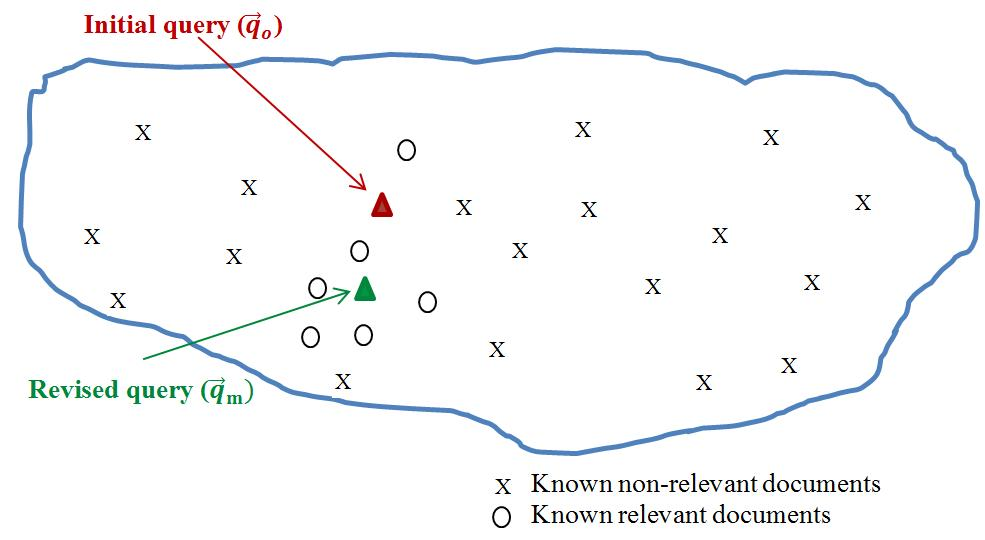
\includegraphics[width=0.65\textwidth,height=50mm]{figs/rocchio.jpg}
   \caption{Rocchio algorithm for relevance feedback. Some documents have been labelled as relevant and irrelevant and the initial query vector is moved in response to this feedback~\citep{manning2008introduction}.}  
   \label{fig:rocchio} 
\end{figure}
\FloatBarrier 
%\noindent
\textit{The Rocchio Algorithm for Relevance Feedback}: The Rocchio
algorithm \citep{Salton1971} is a classic algorithm of relevance feedback
used mainly for query expansion. In brief, it provides a method of
incorporating relevance feedback information into the vector space
model representing a query~\citep{manning2008introduction}. 
The Rocchio algorithm is used to modify the query by the partial knowledge of known relevant and irrelevant~\footnote{In this thesis, we use irrelevant and non-relevant interchangeably for documents that are not relevant to the query.} documents; the goal is to move the query closer to the centroid of the relevant documents but further from irrelevant documents (Figure \ref{fig:rocchio}). The modified query $ \vec{q}_m $ is:
%\[ 
\begin{equation}
\label{eq:rocchio}
 \vec{q}_{m} = \alpha  \vec{q}_{0} + \beta\frac{1}{|D_{r}|}\sum\limits_{\vec{d_{j}}\in D_{r}} \vec{d_{j}} - \gamma\frac{1}{|D_{irr}|}\sum\limits_{\vec{d_{j}}\in D_{irr}} \vec{d_{j}},
  \end{equation}
 %\tag{2.1}\label{eq:rocchio}
 %\]  
where $ q_{0} $ is the original query vector; $ D_{r} $ and $ D_{irr} $ are the set of known relevant and irrelevant documents, respectively; and $ \alpha $, $ \beta $, and $ \gamma $ are weights attached to each term. These control the balance between trusting the judged document set versus the query: if we have a lot of judged documents, we
would like higher $ \beta $ and $ \gamma $~\citep{manning2008introduction}. 

PRF is typically used in Rocchio algorithm. However, it is important to distinguish between good expansion terms and bad ones. Distinguishing between expansion terms only based on their distribution in the feedback documents (i.e., extracting the most frequent terms) and in the whole collection (i.e., extracting the most specific terms) is not sufficient. It can be considered as a term classification problem to separate good expansion terms from others directly according to their potential impact on the retrieval effectiveness; hence, we can apply supervised learning methods for term selection. Classifiers like support vector machines (SVM)~\citep{cao2008selecting}, Na\"ive Bayes and Logistic Regression~\citep{he2009finding} can be used to classify terms and feedback documents.  
\paragraph{Query Expansion by External Resources}
\ \\
The most common form of query expansion is a global analysis, using dictionaries, WordNet, Wikipedia, or other thesaurus. For each term $ t $ in a query, the query can be automatically expanded with synonyms and related words of $ t $ from the thesaurus. Use of a thesaurus can be combined with ideas of term weighting; for instance, one might weight added terms less than original query terms~\citep{manning2008introduction}.
%
%\subsection{Query Reduction (QR)}
%%In general, retrieval effectiveness for long queries is often lower than retrieval effectiveness for shorter keyword queries because the additional information provided in verbose queries is more likely to confuse current search engines rather than help them. Query reduction (QR), a technique for dropping unnecessary query terms from long queries, improves the performance. 

A common approach to reduce verbose queries is selecting a subset of a long query (or sub-query). A search engine performs more precisely when just the key concepts are used as a query rather than a long query. Hence, the identification of the key query concepts has a positive impact on the retrieval performance for verbose queries. Extracting the key query concepts can be done by learning to identify key concepts in long queries using a variety of features~\citep{bendersky2008discovering}. We can choose effective subsets in a query by analysing all the subsets of terms from the original query (sub-queries), and identifying the most promising sub-query to replace the original long query. For ranking sub-queries, an algorithm based on the SVM classification is used~\citep{kumaran2009reducing}. In this approach, the quality of query reduction depends on the performance of the predictor and ranking algorithm~\citep{balasubramanian2010exploring}. 

As the other approach, we can use query term ranking techniques to select effective terms from a verbose query by ranking them. A vast number of rankings are possible given different settings of individual term weights; for example, we can train a regression model to weight all query words of a verbose query~\citep{lease2009regression}. We can also assign weights to concepts by learning the importance of concepts underlying
the verbose query~\citep{bendersky2010learning}.

%%\subsubsection{Query Reformulation}
%%\input{query_reform}
%
%\subsection{IR Evaluation Metrics}
%%A retrieval system is evaluated considering a set of relevance judgements, a binary assessment of either \textit{relevant} or \textit{irrelevant} for each query-document pair. An ideal retrieval system can retrieve all relevant documents. Table \ref{tab:contengency} is the contingency table, where:\\\\
\textit{True Positive (tp)}: documents which are relevant and the system retrieves them.\\
\textit{False Negative (fn)}: documents which are relevant but the system does not retrieve them. \\
\textit{False Positive (fp)}: documents which are non-relevant but the system retrieves them.\\
\textit{True Negative (tn)}: documents which are non-relevant and the system does not retrieve them. 
\begin{table*}[htpb]
  \centering
  \input table/contingency.tex
  \caption{Contingency table.}
  \label{tab:contengency}
\end{table*}
\FloatBarrier 
\paragraph{Precision and Recall}
\ \\
Precision and recall are the most frequent and basic measures for information retrieval effectiveness. They are calculated with respect to what IR system returns as a set of documents for a query.\\
\textit{Precision (P)} is the fraction of retrieved documents that are relevant:
\[
Precision (P)=\frac{\sharp(relevant \: items \: retrieved)}{\sharp(retrieved \: items)}=\frac{tp}{tp+fp}=P(relevant|retrieved)
\]
\textit{Recall (R)} is the fraction of relevant documents that are retrieved:
\[
Recall (R)=\frac{\sharp(relevant \: items \: retrieved)}{\sharp(relevant \: items)}=\frac{tp}{tp+fn}=P(retrieved|relevant)
\]
For many prominent applications, particularly web search, good results on the first page or the first three pages are important than all relevant documents. So, they wish to look at precisions and recalls over a series of different rank cut-offs rather than to look at the entire retrieved set. This is referred to as ``Precision/Recall at k'', for example ``Precision/Recall at 10''. 
\begin{equation}
precision@k=\frac{\sharp(documents \: retrieved \: and \: relevant \: up \: to \: rank \: k)}{k}
\end{equation}
\begin{equation}
recall@k=\frac{\sharp(documents \: retrieved \: and \: relevant \: up \: to \: rank \: k)}{\sharp(documents \: relevant)}
\end{equation}
\paragraph{Average Precision and Mean Average Precision (MAP) }
\ \\
We can measure MAP by calculating Average Precision on retrieval results. Average Precision is the average of precision at each point where a relevant document is found is computed as:
\begin{equation}
Avg. \: precision=\frac{\sum_{r=1}^{N}(P(r)\times rel(r))}{n}
\end{equation}
\noindent
where $ r $ is the rank, $ N $ the number of documents retrieved, $ rel(r) $ a binary function of the document relevance at a given rank, $ P(r) $ is precision at a given cut-off rank $ r $, and $ n $ is the total number of relevant documents.

Then, for a given set of queries, $ Q $, $ MAP $ can be calculated by:
\begin{equation}
MAP(Q)=\frac{\sum_{q\in Q}Avg. \: precision(q)}{|Q|}
\end{equation}
\noindent
where $ q $ is a query in a set of queries $ Q $.
%
%%------------------- Patent-specific IR ---------------------
%
%\section{Patent-specific IR}
%\label{subsec:patentir}
%
%\subsection{The Study of Retrievablity for patents}
%%Rerievability is specifically critical in recall oriented applications like patent retrieval or legal settings. In these cases, the focus of a system is to retrieve all documents that are relevant rather than to retrieve a subset of documents that the best satisfy the query intent.
Hence, all documents should at least potentially be retrievable via correct query terms. Designing retrieval systems for recall oriented tasks has been emphasised in recent years~\citep{fujii2007introduction, kontostathis2008effect}. Before designing a new or using an existing retrieval system for recall oriented applications, one needs to analyse the effects of the retrieval system bias as well as the overall retrievability of all documents in the collection using the retrieval function at hand.

In retrievability, we analyse documents specifically with respect to relevant and irrelevant queries to identify whether highly retrievable documents are really highly retrievable, or whether they are simply more accessible from many irrelevant queries rather than from relevant queries. Experiments show that about 90\% of patent documents which are highly retrievable across all types of queries, are not highly retrievable on their relevant query sets~\citep{bashir2009analyzing}.

Experiments with different collections of patent documents suggest that query expansion with pseudo relevance feedback can be used as an effective approach for increasing the findability of individual documents and decreasing the retrieval bias. Pseudo relevance feedback documents are identified using cluster-based~\citep{bashir2009improving} or terms-proximity-based methods~\citep{bashir2010improving}.

Another study~\citep{bache2010improving} analyses the relationship between retrievability and effectiveness-based measures (Precision, MAP). Results show that the two goals of maximising access and maximising performance are quite compatible. They further conclude that a reasonably good retrieval performance can be obtained by selecting parameters that maximise retrievability (i.e., when there is the least inequality between documents according to Gini coefficient given the retrievability values). Their results support the hypothesis that retrieval functions can be effectively tuned using a retrievability-based measure without recourse to relevance judgments, making it an attractive alternative for automatic evaluation.

%
%\subsection{Query Formulation}
%%%Query or topic is the the request for information in any retrieval system. An effective query can lead in retrieving the required information. Queries formulated by users are not usually optimal for retrieval process, therefore, they need to be transformed by techniques such as query expansion or query reduction. 
The patent prior art search begins with a full patent application as a query. A full text as a query is a challenge compared to a classical IR, since it is not focused on the information that the user needs. In order to achieve good retrieval results, it is important to extract the best representative text with the proper weights. Therefore, query generation based on query document is essential to reduce the difficulty of formulating effective queries by users. 
%The query created before the retrieval can be modified or enhanced after retrieval. In this section, the initial query formulation will be discussed and in the next section, post-retrieval query reformulation will be covered. 
\\\\
\textbf{Which fields in patent application are more effective to extract query terms}
\ \\
A special characteristic of patent documents is their structural information. They mainly have different fields such as title, abstract, description, and claims. Different fields use different type of language for describing the invention. Abstract and description use more technical terminology while claim field usually uses a legal jargon. Structured indexing keeps the field structure in the index, which allows searching specific fields instead of searching in full document. Separate fields for meta-data (Section \ref{sec:metadata} ) like IPC code and author can help to retrieval effectiveness~\citep{magdy2010exploring}. 

Early patent search tasks mainly considered claims to build the query, the same as what examiners start the novelty process~\citep{konishi2005query, takaki2004associative, mase2005proposal, fujii2007enhancing}, whereas recent works have showed that building queries from description field is more useful in patent retrieval (considering background summary in US patents equivalent to description field in European patents.)~\citep{xue2009transforming, xue2009automatic, mahdabi2011building}. Another research showed that extracting terms according to $ log(tf)idf $ scores from every field of the query patent, and giving higher importance to terms extracted from the abstract, claims, and description fields than to terms extracted from the title field, is an effective way of constructing a search query~\citep{cetintas2012effective}. The other experiment showed that discarding description from query improves MAP up to 30\% because the description contains more noise than information~\citep{gobeill2010simple}. They also showed that claims are more informative and title is poorly informative in retrieval.   


\paragraph{Using Phrases instead of Terms}
\ \\
Most of query formulation techniques rely on terms, but encouraging results have been obtained using phrases recently~\citep{becks2010phrases}. Early results demonstrated that an NLP-based grouping of terms can increase the performance compared to the bag-of-words approach, though the increase is smaller than in a non-patent collection~\citep{osborn1997evaluating}. Another task could improve retrieval effectiveness by adding syntactic phrases in the form of dependency triples, to a bag-of-words representation~\citep{d2011combining}. Key Phrase Extraction (KPE) algorithms is another way to form a query based on phrases. A list of phrases, generated by a KPE algorithm, can succinctly represent a complex and lengthy patent. ~\citep{verma2011applying}.

\paragraph{Diverse Query Generation}
\ \\
In this approach, the focus is on generating diverse queries that can improve overall retrieval effectiveness in sessions rather than generating a single best query that can retrieve more relevant documents from a single retrieval result (i.e., more relevant documents in aggregated retrieval results obtained by multiple queries in a session). Diverse query generation is important because query documents typically contain several different aspects (or topics) and different types of relevant documents may be related to these aspects. To identify aspects, 500 top terms based on their tf-idf rank, are clustered into $ n $ sets with respect to their similarity. Each distinct sets of terms represents one query aspect, then top $ k $ retrieved documents for each sub-query consider as pseudo-relevant documents (PRD) and those ranked below the top $ k $ are non-relevant documents (NRD). Then the query is generated by decision tree. ~\citep{kim2014searching, kim2014diversifying}.
%
%\subsection{Query Expansion for Patents}
%%Although a query is very long in patent prior art search, a significant term mismatch between queries and relevant documents has reported in~\citep{roda2010clef, magdy2010exploring}. The QE is a suggested solution to cope with the term mismatch problem; however, most of the QE techniques were ineffective to improve the performance in patent domain~\citep{kishida2003experiment, konishi2005query}. We review previous works on the QE techniques for the patent search here.
\paragraph{Query Expansion by Pseudo Relevance Feedback}
\ \\
Previous studies~\citep{magdy2011study} have discussed that PRF is ineffective for patent prior art search. Since the retrieval effectiveness is low at initial retrieval, the assumption that top $ k $ documents are relevant is invalid and leads in adding noise to the query; hence, the improvement using PRF is insignificant. The solutions proposed to cope with this problem are as follows:
\begin{list}{-}{}
\item \textbf{Selecting documents for PRF based on cluster analysis:} In this approach, a document that can cluster lots of high similar documents is considered relevant and a document that has no nearest neighbour or some neighbours with low similarity is considered irrelevant~\citep{lee2008cluster}. In patent domain, where there is a large vocabulary diversity for expressing an invention, the idea can be improved by intra-cluster similarity rather than only on the basis of their size~\citep{bashir2009improving}. 
\item \textbf{Selecting patents for PRF based on their similarity with query patent via specific terms:} In this approach, patents for PRF are identified based on their similarity with query patents over a subset of terms, rather than the overall document similarity. The success of this approach highly depends on selecting appropriate terms from patent query, which produce the best PRF candidates that can help in improving retrievability during QE~\citep{bashir2010improving}. Experiments show a significant improvement for Gini coefficient, which is used to measure retrievability, but there is no report on other main measures (e.g., MAP and recall).
\item \textbf{Identyfying expansion terms: } 
\ \\
Term proximity information can be used to identify expansion terms. Given a patent query, first, an initial query is generated by taking, for example, claim terms; then a query-specific lexicon based on definitions of the IPC is created.
Among many terms in the lexicon, only expansion terms identified by two adjacency operators used in patent examination\footnote{Patent examiners use term proximity heuristics in their
searches in Boolean retrieval model in order to reward a
document where the matched query terms occur close to
each other. Two forms of adjacency operators are used in
Boolean retrieval model to address proximity. `ADJn' operator which searches for terms within \textit{n} words proximity in
the order specified, and `NEARn' operator, which searches
for the terms within \textit{n} words, in either order.} (i.e., `ADJn' and `NEARn') are used for query expansion~\citep{mahdabi2013leveraging}.
\item \textbf{Predicting the effectiveness of feedback documents: } 
\ \\
In patent retrieval, the MAP is very low at initial retrieval; hence the top retrieved documents are not essentially relevant. 
As a result, there is a high
chance that we use irrelevant documents for expansion in PRF. Recently,
machine learning methods like regression are used to improve the PRF by predicting the effectiveness of a feedback document~\citep{mahdabi2012learning}.
\end{list}
Random indexing to identify terms to use for query expansion~\citep{sahlgren2002english} and expansion using noun phrases~\citep{mahdabi2012automatic} are the other techniques to improve the effectiveness of standard query expansion for prior art search. 
\paragraph{Query Expansion by External Resources}
\ \\
Some external resources like WordNet~\citep{miller1990introduction}, which were reported to improve retrieval effectiveness in several IR research investigations, show insignificant change to overall retrieval effectiveness, but a degree of improvement for some topics in patent domain. \cite{magdy2011study} applied the idea of automatically generating the synonyms set (SynSet) using parallel manual translations to create possible synonyms sets (in CLEF-IP collection, some sections in some patents are translated into three languages: English, French, and German). Although this idea presents better results compared to WordNet, there is still a little improvement in retrieval effectiveness. The only QE task, which achieves the best results, uses a combination of PRF and QE with translation of terms and phrases from German and French~\citep{jochim2011expanding}.

%
%\subsection{Query Reduction for Patents}
%%Query reduction is a solution for problems with using a full verbose patent as a query: it is not focused on information needed by the user, and a verbose query may cover more than one topic.

\begin{list}{-}{}

\item \textbf{Query Segmentation :} Decomposing each patent query into coherent sub-topics segments-using TextTiling~\citep{hearst1997texttiling}-is a solution to make long ambiguous queries focused on the information need. Sub-topic segments can be used as separate queries (query stream) for initial retrieval, then the retrieval results from each of the individual streams are merged to construct the final ranked list for the whole original query. Using each sub-topic as a query stream enables a retrieval model to retrieve related documents from the collection in a more precise way and also allow the PRF algorithm to work on a more focused set of pseudo-relevant documents~\citep{takaki2004associative, ganguly2011united}. Another work adapted pseudo relevance feedback for query reduction by decomposing a patent application into constituent text segments and computing the Language Modelling (LM) similarities by calculating the probability of generating each segment from the top ranked documents. The least similar segments from the query removed from the query, hypothesizing that removal of segments most dissimilar to the pseudo-relevant documents can increase the precision of retrieval by removing non-useful context, while still retaining the useful context to achieve high recall as well~\citep{ganguly2011patent}.

\item \textbf{Patent Summarization :} This approach assumes that the patent summary (using TextTiling) reflects the main topic as well as the subtopics of a patent document in a concise manner. Then, language model for the query, collection, and each summary are generated~\citep{mahdabi2011report}. 

\end{list}


%
%%\subsubsection{Query Reformulation for Patents}
%%\input{query-reform-p}
%
%\subsection{The Use of Metadata}
%%The main textual content of patent documents is known to be difficult to process with traditional text processing and text retrieval techniques, but patents contain additional material, such as: tables, mathematical and chemical formulas, citations, technical drawing, meta-data, e.g., applicant, inventor, Intentional Patent Classification (IPC) codes, and publication date, that can be used to improve the retrieval. In this section, the use of patent meta-data to improve the retrieval has been explained.
\paragraph{The Use of Citation}
\ \\
The most successful use of metadata to date is the citation lists in order to learn patterns of relevance ~\citep{lupu2013patent}. The patent collection is a very dense network of citations creating a set of interrelations particularly interesting to exploit during a prior art search. The large majority of patents are continuations of previous works and patents. The citation relations make this development process
visible. Similarly, fundamental patents which open new technologies sub-fields are exceptional but tends to be cited very frequently in the whole sub-field during years. Citation graph of a patent collection is used for identifying patent thickets, i.e. the patent portfolios of several companies overlapping on a similar technical aspect. Related patents can be inferred from the overall citation network of a patent collection. If a new patent applicant belonging to this patent ticket appears, it is very likely that the most relevant prior art documents are already
present in this patent thicket~\citep{lopez2009multiple}.

The patents cited in the description of the topic patent are used as relevant documents, because citations are usually prior arts for a citing patent. Only citations which are in the collection can be helpful in the retrieval process. The idea of \textit{PageRank}-identifying authoritative pages by analysing hyperlink structure on World Wide Web\_ can be used for citations. A patent, which is cited by a large number of other patents, is more important. Text-based and citation-based scores combined to compute the ranking score for documents~\citep{fujii2007enhancing, fujii2007integrating}.

Citation texts for patents are a whole paragraph. Therefore, for each patent document presented and cited in the collection, the entire paragraph of citation can be appended to the textual material of the cited patent. A boolean feature uses to indicate weather a cited patent in query patent has retrieved, then this document can get a higher weight at any future post-ranking process. Due to the limited number of citation texts, this approach showed just a trivial improvement~\citep{lopez2009multiple}. However, citation information does not always presented in the patent application and this method can not be used in real life patent search and initial citations by the applicants may not consider relevant by patent examiners~\citep{magdy2010applying, magdy2011simple}. 

Similar tasks also indicated improvement in 'MAP' and 'Recal' using citations in patent retrieval~\citep{gobeill2010simple, gurulingappa2010prior}. 
\paragraph{The Use of IPC Codes}
\ \\
Patents are classified by the patent offices into large hierarchical classification schemes based on their area of technology. The use of patent
classification has two major benefits. The first is that the classifications provide access to concepts rather than words, such that even
if the same word or phrase is commonly used in two technology areas, patent classifications will provide the context of its use. In effect, they
allow the search space of patents to be reduced, by allowing the user to exclude from the search process patents in classes not related to
the search topic at hand~\citep{lopez2010patatras}. The second major benefit is the language independence provided by classifications, as classification symbols can be mapped to multiple languages~\citep{DBLP:conf/clef/DhondtV10}. This allows patent searchers to conduct reasonably effective retrieval even in languages that they do not understand. All previous works, considered IPC code in their search, reported improvement in retrieval effectiveness~\citep{harris2010comparison, harris2011using, harris2009role, fujita2005revisiting, graf2010knowledge, herbert2010prior, kang2007cluster, verma2011applying}. It has also reported that using complete IPC code leads in better results than just 4-digit code~\citep{ gobeill2010simple}.
\paragraph{The Use of Images}
\ \\
For the purposes of the search for innovation, we are interested in all forms of information. Some technology areas rely information present in images (flowcharts and diagrams), so, beyond text data, image processing tasks also can contribute to the search. Graph-based measure has a higher discriminative power, but higher computational costs than the text-based measures~\citep{lupu2013evaluating}.

%\label{sec:metadata}
%
%\subsection{Multilinguality}
%%The interest in multilingual patent search arises from their international and multilingual nature (the European patent office-EPO-makes patent text available in three languages: English, French, and German). Patents on the same topic may be published in different countries in different languages, and it is important for patent examiners to be able to locate relevant existing patents whatever language they are published in. Therefore an important topic in patent retrieval is Cross-Language Information Retrieval (CLIR), where the topic is a patent application in one language and the objective is to find relevant prior-art patents in another language ~\citep{lupu2013patent,joho2010survey, roda2010clef, DBLP:conf/clef/PiroiLHSMF12}. In recent years machine
translation (MT) has become established as the dominant technique for translation in CLIR, which usually achieve better CLIR effectiveness than dictionary-based translation (DBT) methods. However, translation using MT is time consuming and resource intensive for cross language patent retrieval (CLPR), where the query text can often take the form of a full patent application running to tens of pages. Applying IR text pre-processing like stop word removal and stemming to the MT training corpus prior to the training phase can lead to a significant decrease in the MT computational~\citep{magdy2013studying}.



%
%\subsection{Multi-stage Retrieval}
%It is common to use patent meta-data and non-textual features as pre and post processing steps of text-based retrieval techniques~\citep{lopez2009multiple}. Many patent retrieval tasks re-rank the top retrieved documents from initial retrieval stage based on additional patent feature ~\citep{lopez2010experiments}, claim structure ~\citep{mase2005proposal}, and considering IPC information of patent and its neighbours to retrieve similar patents~\citep{verma2011exploring}. 
%
%\subsection{Evaluation Metrics for Patent Retrieval}
%%The simplest solution to measure the performance in a recall focused IR task is to evaluate the recall, however, it fails to reflect how early a system retrieves the relevant documents and without precision, returning a perfect recall is invalid~\citep{Suominen08t.:critical}. Although recall is the objective for such applications, the score should be able to distinguish between systems that retrieve relevant documents earlier than those that retrieve them later. For recall-oriented IR applications, the problem is viewed as a ranking problem with a cut-off for a maximum number of documents to be checked $ N_{\max} $.\\\\
\textbf{Patent Retrieval Evaluation Score}
\ \\
\begin{figure}[t!]
   \centering
%   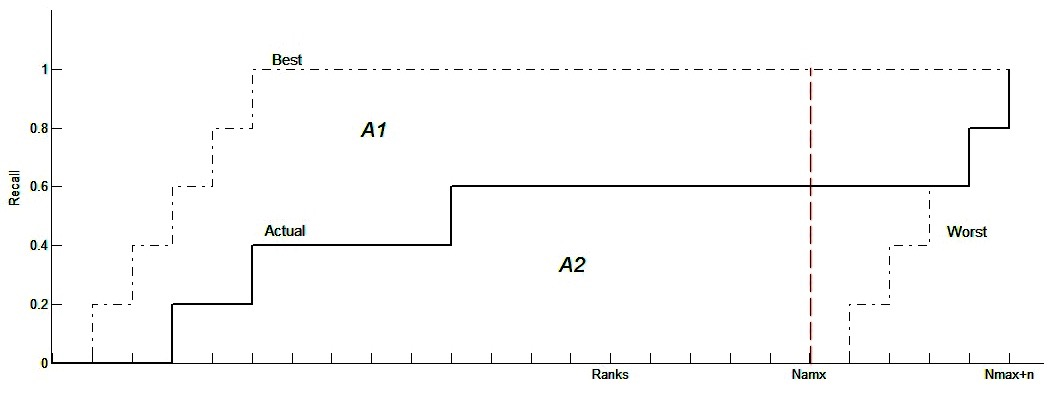
\includegraphics[width=1\textwidth,height=50mm]{figs/pres.jpg}
   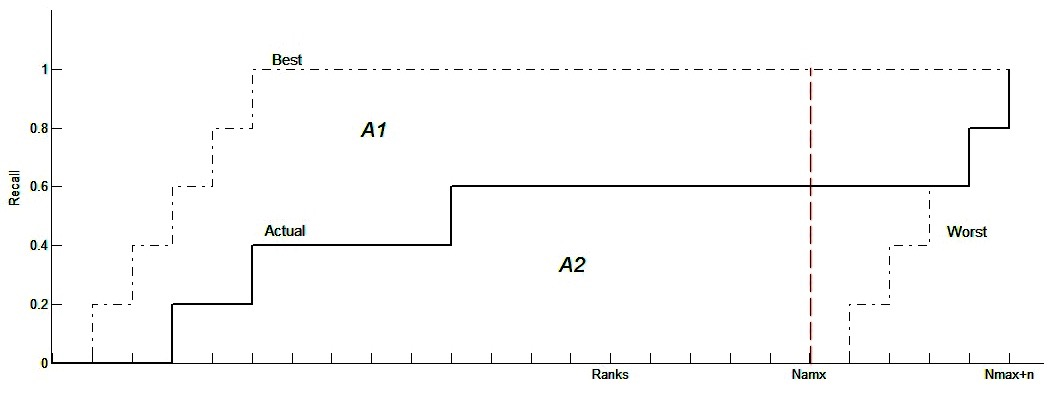
\includegraphics[scale=.37]{figs/pres.jpg}
   \caption{PRES curve is bounded between the best case and the new defined worst case~\citep{magdy2010pres}.}  
   \label{fig:pres} 
\end{figure}
%\FloatBarrier 
Patent retrieval evaluation score (PRES)~\citep{magdy2010pres} is a novel metric for evaluating recall-oriented IR applications, which derived from the normalised recall measure ($ R_{norm} $). It measures the ability of a system to retrieve all known relevant documents earlier in the ranked list. Unlike MAP and recall, PRES is dependent on the relative effort exerted by users to find relevant documents. This is mapped by $ N_{\max} $ (Equation \ref{eq:pres}), which is an adjustable parameter that can be set by users and indicates the maximum number of documents they are willing to check in the ranked list. PRES measures the effectiveness of ranking documents relative to the best and worst ranking cases, where the best ranking case is retrieving all relevant documents at the top of the list, and the worst is to retrieve all the relevant documents just after the maximum number of documents to
be checked by the user ($ N_{\max} $). The idea behind this assumption is that getting any relevant document after $ N_{\max} $ leads to it being missed by the user, and getting all relevant documents after max leads to a zero recall, which is the theoretical worst case scenario. 
%Figure 1 shows an illustrative graph of how to calculate PRES, where 
PRES is the area between the actual and worst cases ($ A_{2} $) divided by the area between the best and worst cases ($ A_{1}+A_{2} $).
$ N_{\max} $ introduces a new definition to the quality of ranking of relevant results, as the ranks of results are relative to the value of $ N_{\max} $. Any relevant document not retrieved in the top N max is assumed to be the worst case (Figure~\ref{fig:pres}).
For example, getting a relevant document at the rank 10 will be very good when $ N_{\max}=1000 $, good when $ N_{\max}=100 $, but bad when $ N_{\max}=15 $, and very bad when $ N_{\max}=10 $. Systems with a higher recall can achieve a lower PRES value when compared to systems with a lower recall but a better average ranking. The PRES value varies from $ R $ to $ \frac{nR^{2}}{N_{\max}} $, where $ R $ is the recall, according to the average quality of ranking of relevant documents.
\begin{equation}
\label{eq:pres}
PRES=\frac{A_{2}}{A_{1}+A_{2}}=1-\frac{\frac{\sum r_{i}}{n}-\frac{n+1}{2}}{N_{\max}},
\end{equation}
where $ r_{i} $ is the rank at which the $ i $th relevant document is retrieved, $ N_{\max} $ is the maximum number of retrieved documents to be checked by the user (i.e. the cut-off number of retrieved documents) and $ n $ is the total number of relevant documents.


%At the begging of each chapter, please introduce the motivation and high-level
%picture of the chapter. You also have to introduce sections in the
%chapter. \\
%
%
%Section~\ref{sec:motivation} xxxx.\\
%
%
%Section~\ref{sec:relatedwork} yyyy.\\
%
%
%\section{Motivation}
%\label{sec:motivation}
%
%
%\section{Related work}
%\label{sec:relatedwork}
%You may reference other papers. For example: 
%Generational garbage collection~\citep{LH:83,Moon:84,Ungar:84} is perhaps the
%single most important advance in garbage collection since the first collectors
%were developed in the early 1960s. (doi: "doi" should just be the doi part, not
%the full URL, and it will be made to link to dx.doi.org and resolve.
%shortname: gives an optional short name for a conference like PLDI '08.)
%
%
%
%
%
%\section{Summary}
%Summary what you discussed in this chapter, and mention the story in next
%chapter. Readers should roughly understand what your thesis takes about by only reading
%words at the beginning and the end (Summary) of each chapter.
%


